% !TeX spellcheck = pt_BR
\documentclass[tese_patricia]{subfiles}
\begin{document}

% ---------------------------------------------------------- 
% Métodos de malhas sobrepostas
% ----------------------------------------------------------
\chapter[Análise isogeométrica aplicada à Dinâmica dos Fluidos Computacional]{Análise isogeométrica aplicada à Dinâmica dos Fluidos Computacional} \label{capitulo:Cap3}
% ----------------------------------------------------------

%\nomenclature[C,01]{$p$}{Grau das funções base na direção paramétrica $\xsi$;}
%\nomenclature[C,02]{$\xsi$}{Vetor de \textit{knots} na direção paramétrica $\xsi$;}
%\nomenclature[C,03]{$\xsi$}{Uma das direções paramémtricas nas quais as funções base são definidas;}
%\nomenclature[C,04]{$n$}{Número de funções base na direção paramétrica $\xsi$ ;}
%\nomenclature[C,05]{$N$}{Função base \textit {B-Spline} na direção paramétrica $\xsi$ ;}
%\nomenclature[C,06]{$\CP$}{Pontos de controle que descrevem a geometria \textit{B-Spline} ou NURBS;}
%\nomenclature[C,07]{$\mathbf{C}$}{Curva \textit {B-Spline} ou NURBS;}
%\nomenclature[C,08]{$m$}{Grau das funções base na direção paramétrica $\eta$;}
%\nomenclature[C,09]{$\mathcal{H}$}{Vetor de \textit{knots} na direção paramétrica $\eta$;}
%\nomenclature[C,10]{$q$}{Número de funções base na direção paramétrica $\eta$ ;}
%\nomenclature[C,11]{$\eta$}{Uma das direções paramémtricas nas quais as funções base são definidas;}
%\nomenclature[C,12]{$M$}{Função base \textit {B-Spline} na direção paramétrica $\eta$ ;}
%\nomenclature[C,13]{$\mathbf{S}$}{Superfície \textit {B-Spline} ou NURBS;}
%\nomenclature[C,14]{$\hat{N}$}{Função \textit {B-Spline} fruto do produto tensorial entre funções base descritas em um espaço paramétrico qualquer;}
%\nomenclature[C,15]{$L$}{Função base \textit {B-Spline} na direção paramétrica $\zeta$ ;}
%\nomenclature[C,16]{$r$}{Grau das funções base na direção paramétrica $\zeta$;}
%\nomenclature[C,17]{$\mathcal{Z}$}{Vetor de \textit{knots} na direção paramétrica $\zeta$;}
%\nomenclature[C,18]{$\zeta$}{Uma das direções paramémtricas nas quais as funções base são definidas;}
%\nomenclature[C,19]{$l$}{Número de funções base na direção paramétrica $\zeta$ ;}
%\nomenclature[C,20]{$\mathbf{T}$}{Sólido \textit {B-Spline} ou NURBS;}
%\nomenclature[C,21]{$\mathbf{C}^{w}$}{Curva \textit{B-Spline} no $\realspace^{d+1}$ cuja projeção transformativa gera uma curva \mathbf{C} no $\realspace^{d}$;}
%\nomenclature[C,22]{$R$}{Função base NURBS;}
%\nomenclature[C,23]{$w$}{Peso respectivo a um ponto de controle;}
%\nomenclature[C,24]{$\mathbf{\hat{\xsi}}$}{Coordenadas do espaço parental, no qual realiza-se a integração numérica;}
%\nomenclature[C,25]{$\hat{\xsi}$}{Uma das direções do espaço parental;}
%\nomenclature[C,26]{$\hat{\eta}$}{Uma das direções do espaço parental;}
%\nomenclature[C,27]{$\hat{\zeta}$}{Uma das direções do espaço parental;}
%\nomenclature[C,28]{$\tilde{\Omega^{e}}$}{Domínio de uma célula no espaço paramétrico;}
%\nomenclature[C,29]{$\hat{\Omega^{e}}$}{Domínio de um uma célula o no espaço parental;}
%\nomenclature[C,30]{$h$}{Dimensão na direção $y$ da entrada do perfil parabólico no problema do escoamento sobre canal com degrau;}
%\nomenclature[C,31]{$s$}{Dimensão  na direção $y$ do degrau que compõe o problema do escoamento sobre canal com degrau;}
%\nomenclature[C,32]{$x_{e}$}{Dimensão na direção $x$  do degrau que compõe o problema do escoamento sobre canal com degrau;}
%\nomenclature[C,33]{$x_{f}$}{Dimensão na direção $x$  do \textit{patch} $P1$ do problema do escoamento sobre canal com degrau;}
%\nomenclature[C,34]{$x_{t}$}{Dimensão do canal após o degrau na direção $x$ do problema do escoamento sobre canal com degrau;}
%\nomenclature[C,35]{$V_{max}$}{Velocidade máxima do perfil parabólico na entrada do problema do escoamento sobre canal com degrau;}
%\nomenclature[C,36]{$x_{r}$}{Dimensão do vórtice primário que se forma no problema de escoamento sobre canal com degrau;}
%\nomenclature[C,37]{$P_{i}$}{Patch de número $i$;}


A Análise Isogeométrica (IGA) é uma técnica numérica introduzida por \citeonline{HughesCB:2005} para obtenção de soluções aproximadas de equações diferenciais. O método pode ser entendido como uma generalização do método dos elementos finitos clássicos a partir do uso de funções base especiais. 

Na Análise Isogeométrica, as funções base escolhidas na discretização da geometria do problema e de suas variáveis são aquelas utilizadas nos sistemas CAD, sendo as funções do tipo NURBS as mais aplicadas (ver, por exemplo, \citeonline{PiegT:1996}). O grande impulso para o desenvolvimento da técnica foi proporcionar a integração entre a engenharia de \textit{design}, com modelos baseados em CAD, e as simulações numéricas, com modelos principalmente baseados no MEF, de forma que ambas trabalhem com somente um modelo geométrico.

Além disso, a IGA apresenta vantagens significativas, uma vez que permite a representação exata de diversas geometrias comuns, como seções cônicas, círculos, cilindros, esferas e elipsoides, além de dispor de algoritmos eficientes e estáveis para a geração de objetos NURBS. As funções NURBS, em particular, possuem propriedades matemáticas que as tornam adequadas para aplicações numéricas, destacando-se a elevada suavidade — com continuidade 
$p-1$  nas interfaces entre elementos, sendo $p$ o grau das funções —, a alta capacidade de aproximação e a possibilidade de refinamento local por meio da inserção de \textit{knots}, que correspondem às coordenadas do espaço paramétrico nas quais as funções são definidas.

{\color{red}REVER ESSE TRECHO QUANDO TERMINAR O CAPÍTULO}.
Nesse capítulo apresenta-se uma breve introdução sobre a IGA, o processo de obtenção das geometrias NURBS e seu uso na descrição das variáveis discretas nas simulações numéricas. As referências bibliográficas que fundamentam esta construção são \citeonline{HughesCB:2005} e \citeonline{PiegT:1996}. Por fim, são apresentados alguns exemplos de sua aplicação em problemas da DFC.

%\vspace{-0.1cm}

\section{Noções Gerais de IGA}

No contexto do MEF isoparamétrico, a formulação é construída a partir da definição de uma malha e de seus elementos, os quais são representados tanto no espaço físico quanto no espaço paramétrico. Cada elemento é caracterizado pelas coordenadas de seus nós, sendo os graus de liberdade do problema associados aos valores das funções de forma interpolados nesses pontos nodais.

Dentro da IGA têm-se duas noções de malha: uma malha de pontos de controle e uma malha física. A malha de pontos de controle é muito semelhante a uma malha de elementos finitos, entretanto, ela não define a geometria, ela é apenas um esqueleto que controla o formato da geometria (ver Fig. \ref{fig:espacos_NURBS}), visto que as funções de forma baseadas em \textit{B-Splines} não são necessariamente interpolatórias. Dessa forma, os graus de liberdade do problema são associados aos pontos de controle, cujas posições não coincidem, necessariamente, com a geometria representada.

\begin{figure}[htb!]
	\centering 
	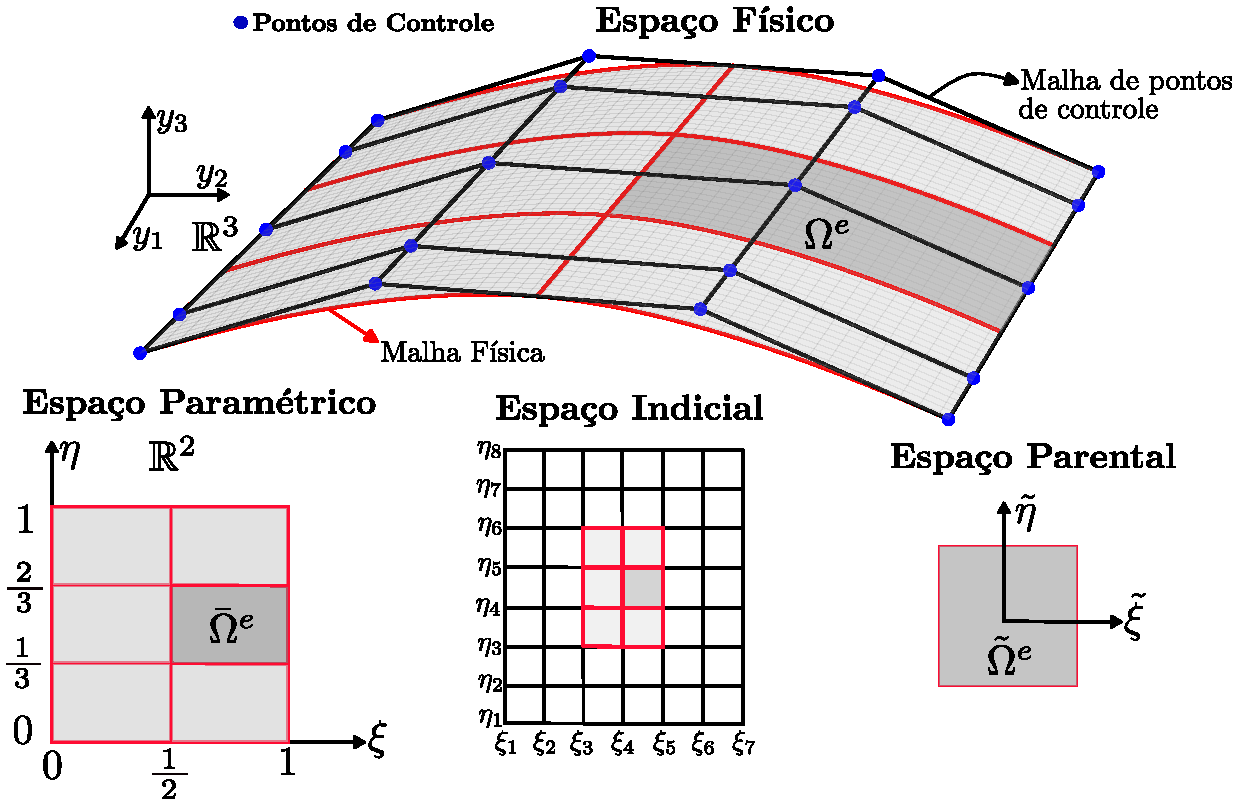
\includegraphics[scale=0.7,trim=0cm 0cm 0cm 0cm, clip=true]{Imagens/Cap3/espacos_NURBS.pdf}	
	\caption{NURBS: espaço físico, espaço paramétrico, espaço indicial e espaço parental}
	\label{fig:espacos_NURBS}
\end{figure}


A malha física representa a geometria discretizada. Dentro da malha física podem ser definidos dois tipos de elementos, um macro-elemento, denominado de \textit{patch}, e o \textit{knot span}, que é o equivalente a um elemento finito e será denominado como célula ao longo desse texto. Cada \textit{patch} é composto por um conjunto de células. Muitas geometrias simples podem ser discretizadas apenas com um \textit{patch}, entretanto, a depender da complexidade da geometria ou de requisitos de parametrização, se torna necessário o uso de um conjunto de \textit{patches}. As células são representações geométricas de linhas, superfícies e volumes nos espaços físicos unidimensional, bidimensional e tridimensional respectivamente.

Cada \textit{patch} e suas respectivas células possuem uma representação no espaço paramétrico (Fig. \ref{fig:espacos_NURBS}), que é o espaço onde as funções base são definidas. O espaço paramétrico, para os casos de funções univariadas, é definido por um \textit{knot vector}, aqui denominado de vetor de \textit{knots}, que é um conjunto de \textit{knots} ou coordenadas paramétricas. As células são constituídas pelo espaço entre dois \textit{knots} consecutivos. O espaço onde se representam todas as células, inclusive as nulas (quando mais de um \textit{knot} ocupa a mesma posição), é chamado de espaço indicial.

Por fim, na análise isogeométrica conta-se ainda com o espaço parental, que é o espaço de integração numérica das funções base, em geral, definido de forma adimensional $[-1, 1]$ dentro de uma célula. Na Fig. \ref{fig:espacos_NURBS} pode-se observar os espaços relatados para uma superfície 3D construída por funções base quadráticas e apenas um \textit{patch}. 

\section{\textit{B-Splines}} \label{capitulo:Cap3:Bsplines}´

Para a construção de uma geometria NURBS, é fundamental compreender as funções base \textit{B-splines} e suas particularidades. Essas funções servem como o ponto de partida para a definição de curvas, superfícies e sólidos NURBS, sendo essenciais para o entendimento da flexibilidade e controle geométrico oferecido por esse modelo. As \textit{B-splines} são funções construídas através de um vetor de coordenadas paramétricas (vetor de \textit{knots}) e que dependem de um conjunto de pontos de controle, sendo esses elementos responsáveis por estabelecer a forma geométrica e o grau de continuidade da curva ou superfície.


\subsection{Vetor de \textit{knots}}

As funções \textit{B-Splines}, utilizadas na construção das NURBS, são definidas em um espaço paramétrico que é comum a um conjunto de células ou \textit{patch}. O espaço paramétrico unidimensional é construído através de um vetor de \textit{knots}, que consiste em um conjunto não decrescente de coordenadas paramétricas, definido como: $\Xsi=\left[\xsi_{0},\xsi_{1},...,\xsi_{n+p+1}\right]$,  sendo que $\xsi_{i}\in \realspace$ e representa a i-ésima coordenada paramétrica  com $i = 0, 1, ..., n+p+1$, e $p$ corresponde ao grau polinomial das funções. O parâmetro 
$n$ equivale ao índice da última função base nesta direção paramétrica, sendo o conjunto de funções base indexado de 
$0 \ \text{a}  \ n$, totalizando $n+1$ funções. Os \textit{knots} definem células no espaço paramétrico, cujos contornos são mapeados pelas funções base para formar a malha no espaço físico. 

O vetor de \textit{knots} pode ser classificado como uniforme, quando as coordenadas paramétricas são igualmente espaçadas, e como não-uniformes, caso contrário.
A multiplicidade de um \textit{knot} pode ser superior a um, influenciando diretamente na continuidade e na forma das funções base, conforme será visto posteriormente.  Os vetores de \textit{knots} conhecidos como abertos, são frequentemente utilizados nas literaturas de CAD, e caracterizam-se por ter a primeira e a última coordenada paramétrica repetidas $p+1$ vezes. Este fato garante que as funções sejam interpolatórias nos extremos do espaço paramétrico e nas bordas entre \textit{patches}, proporcionando, por exemplo, a homogeneidade com respeito às condições de contorno essenciais. 

\subsection{Funções base e suas derivadas}

As funções base \textit{B-Splines} ($\Nb$) univariadas são definidas a partir de um vetor de \textit{knots}, sendo para $p=0$, escritas através da seguinte relação:

\begin{align}
\Nb_{i,0}(\xsi) = \begin{cases} 1 &\mbox{if } \xsi_i\leq\xsi<\xsi_{i+1} \\
0 & \mbox{caso contrário } \end{cases}, \label{eq:bsplines_0}
\end{align}

\noindent enquanto que para funções com $p\geq1$ são definidas como:

\begin{align}
\Nb_{i,p}(\xsi)=\frac{\xsi-\xsi_{i}}{\xsi_{i+p}-\xsi_{i}}\Nb_{i,p-1}(\xsi) + 
\frac{\xsi_{i+p+1}-\xsi}{\xsi_{i+p+1}-\xsi_{i+1}}\Nb_{i+1,p-1}(\xsi), \label{eq:bsplines_n}
\end{align}

\noindent com $i=0,1,...,n$.

Essas equações são conhecidas como a fórmula recursiva de \textit{Cox-de Boor} \cite{Cox1972,DEBOOR1972}. Para funções \textit{B-Splines} de grau $p=0$ ou $p=1$, obtêm-se, respectivamente, as mesmas funções constantes e lineares por partes utilizadas no método dos elementos finitos padrão.

Na Fig.\ref{fig:bspline_funcoes}, pode-se observar funções \textit{B-Splines} quadráticas construídas sobre o vetor de \textit{knots} não-uniforme aberto $\Xsi=\left[0,0,0,1,2,3,3,4,4,4\right]$. A figura evidencia que, devido à repetição de $p+1$ vezes dos \textit{knots} nas extremidades do vetor, as funções base se tornam interpolatórias nesses pontos. Ademais, a presença de um \textit{knot} com multiplicidade 2 em $\xsi=3$ reduz a regularidade da função base nesse ponto, resultando na descontinuidade da sua derivada. Em termos gerais, a continuidade de uma função \textit{B-Spline} em uma coordenada paramétrica é dada por $C^{p-m}$, onde $m$ é a multiplicidade do \textit{knot}.

\begin{figure}[htb!]
	\centering 
	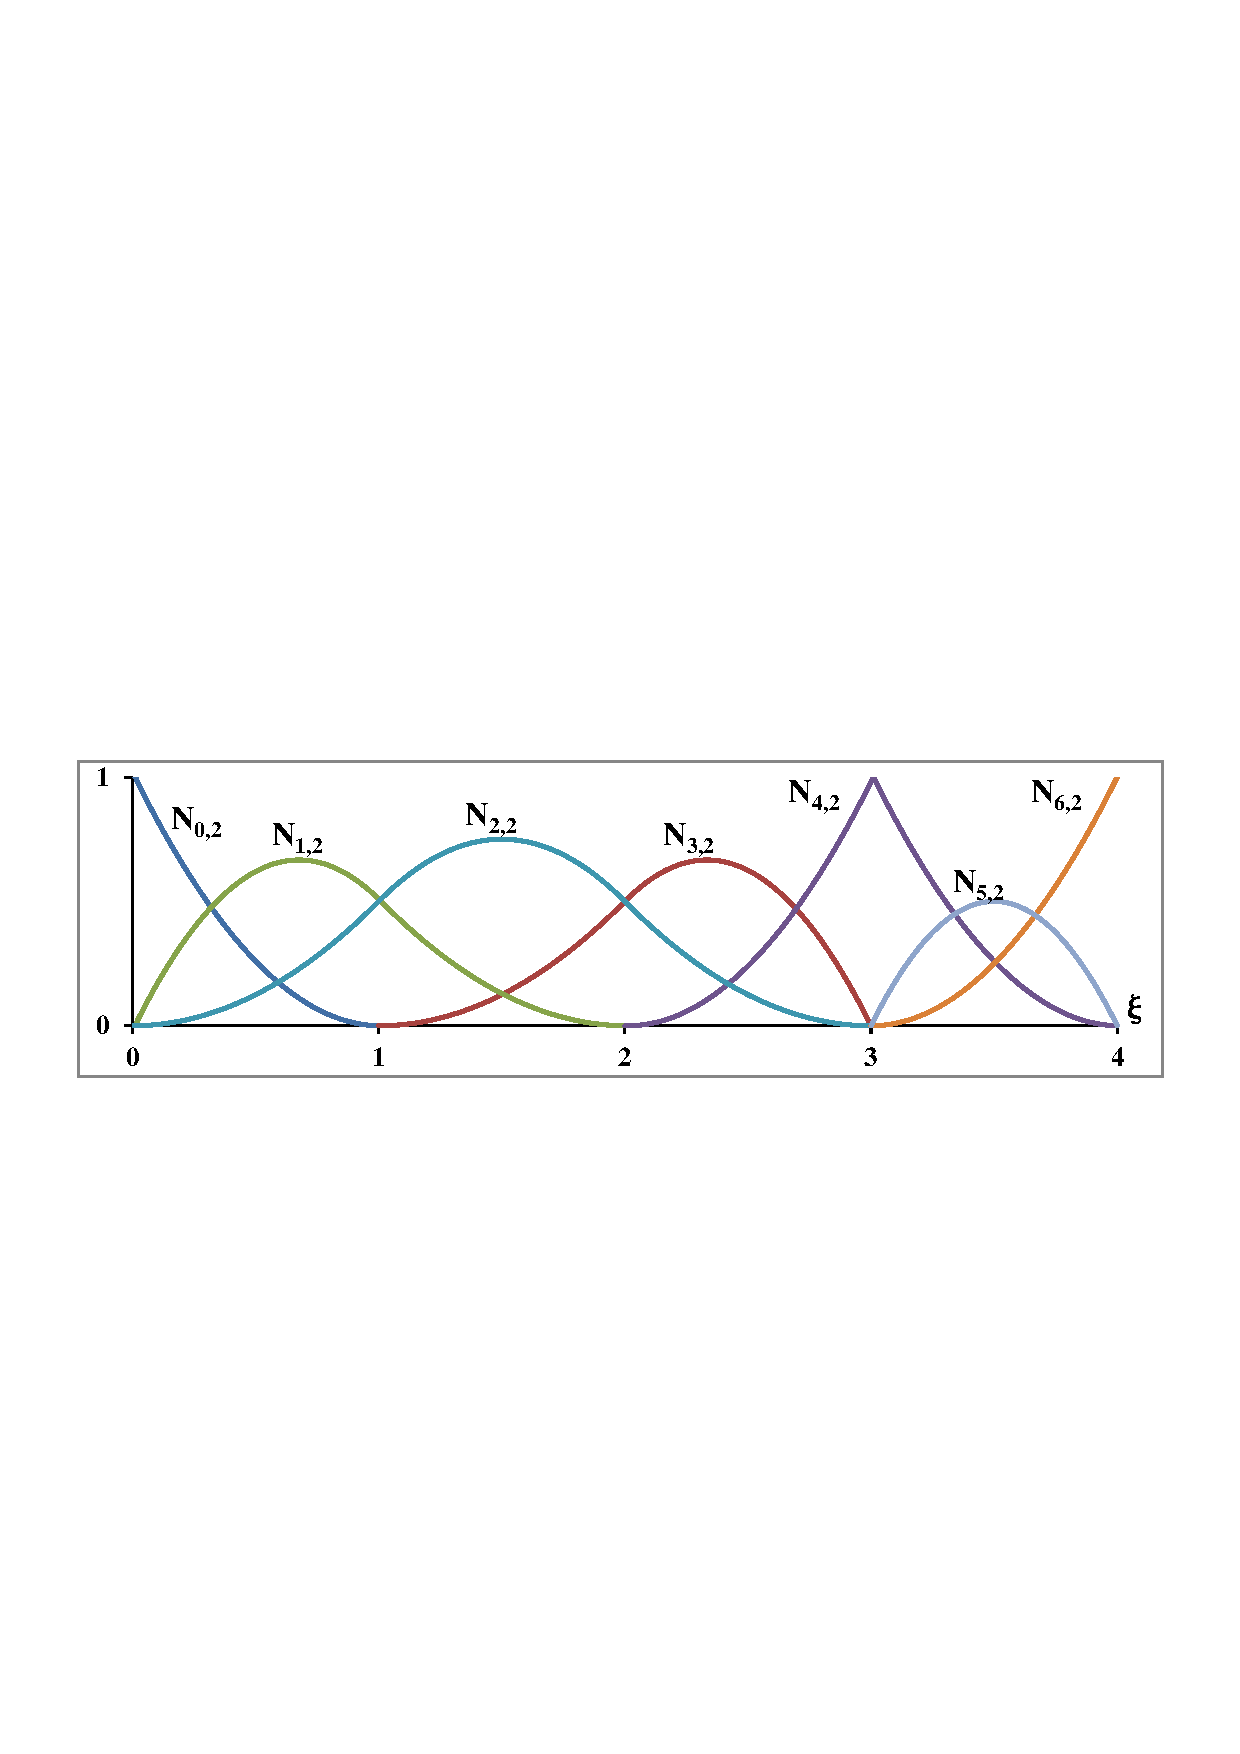
\includegraphics[scale=0.7,trim=1.5cm 11.5cm 1.5cm 13cm, clip=true]{Imagens/Cap3/bspline_funcoes.pdf}	
	\caption{\textit{B-Splines quadráticas}}
	\label{fig:bspline_funcoes}
\end{figure}

As principais propriedades das funções \textit{B-Splines} são:

\begin{itemize}
	\item \textbf{Partição da Unidade}: $\sum_{i=0}^{n}\Nb_{i,p}(\xsi)=1 $;
	\item \textbf{Positividade}: Todas as funções base são positivas, ou seja, $\Nb_{i,p}\geq0$, $\forall\xsi$;
	\item \textbf{Suavidade}: função de ordem $p$ é, em geral, $p-1$ vezes continua no contorno das células;
	\item \textbf{Suporte Compacto}: O suporte de cada $\Nb_{i,p}$ está contido no intervalo $\left[\xsi_i,\xsi_{i+p+1}\right]$, ou seja, em cada célula, apenas $p+1$ funções são não nulas. % Deve-se notar no entanto que, ao se extenderem por vários elementos, o suporte é menos compacto do que para bases formadas por polinômios de lagrange definidos em elementos finitos.
\end{itemize}

A derivada de uma função de forma \textit{B-Spline} pode ser calculada recursivamente em termos de funções base de ordem menor. Considerando uma função de ordem $p$ e vetor de \textit{knots} $\Xsi$, a derivada da i-ésima função de forma pode ser escrita como:

\begin{align}
\frac{\deriv}{\deriv \xsi} \Nb_{i,p}(\xsi) = \frac{p}{\xsi_{i+p} - \xsi_{i}}\Nb_{i,p-1}(\xsi) - \frac{p}{\xsi_{i+p+1} - \xsi_{i+1}}\Nb_{i+1,p-1}(\xsi).
\end{align}

Essa expressão pode ser generalizada para derivadas de ordem superior através de:

\begin{align}
	\frac{\deriv^{k}}{\deriv \xsi^{k}} \Nb_{i,p}(\xsi) = \frac{p!}{\left(p-k\right)!} \sum_{j=0}^{k}{\alpha_{k,j}\Nb_{i+j,p-k}(\xsi)},
\end{align}

sendo $k$ a k-ésima derivada da função $\Nb_{i,p}(\xsi)$ e:

\begin{align}
	\alpha_{0,0} = 1,
\end{align}
\begin{align}
	\alpha_{k,0} = \frac{\alpha_{k-1,0}}{\xsi_{i+p-k+1}-\xsi_{i}},
\end{align}
\begin{align}
	\alpha_{k,j} = \frac{\alpha_{k-1,j}-\alpha_{k-1,j-1}}{\xsi_{i+p+j-k+1}-\xsi_{i+j}} \ \ j=1,...,k-1,
\end{align}
\begin{align}
	\alpha_{k,k} = \frac{-\alpha_{k-1,k-1}}{\xsi_{i+p+1}-\xsi_{i+k}}.
\end{align}

Algoritmos eficientes para a determinação das funções de forma \textit{B-Splines} e de suas derivadas podem ser encontradas em \citeonline{PiegT:1996}.

\subsection{Geometrias \textit{B-Splines}}

Uma curva \textit{B-Spline} é construída a partir da combinação linear entre funções base e um conjunto de pontos de controle. Considerando um conjunto de $n+1$ funções base $\Nb_{i,p}$ e respectivos pontos de controle $\CP_i$ $\in \nrealspace$ com $i = 0,1,...,n$,
uma curva polinomial por partes \textit{B-Spline} univariada é definida como:

\begin{align}
\mathbf{C} =\pos\left(\xsi\right) = \sum_{i=0}^{n}\Nb_{i,p}(\xsi)\CP_i,
\end{align}

\noindent com $y_1$, $y_2$ e $y_3$ as componentes do vetor de coordenadas físicas $\pos$. Utilizando as funções \textit{B-Splines} apresentadas na Fig.\ref{fig:bspline_funcoes} e uma malha de pontos de controle, obtém-se a curva apresentada na Fig.\ref{fig:bspline_malhaPC}. Na Fig.\ref{fig:bspline_curva} pode-se observar as células físicas equivalentes a essa combinação.

\begin{figure}[!htb]
	\centering	
	\subfloat[Malha de pontos de controle\label{fig:bspline_malhaPC}]{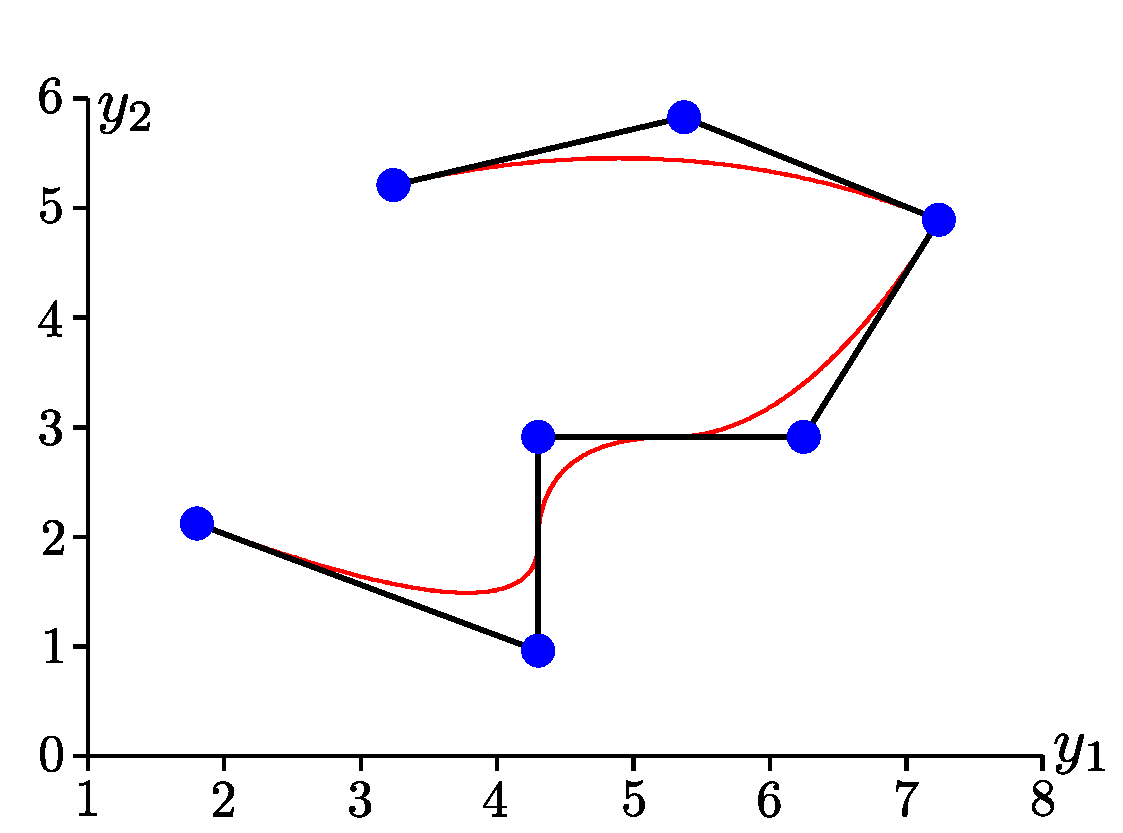
\includegraphics[scale=0.4,trim=0cm 0.0cm 0cm 0cm, clip=true]{Imagens/Cap3/bspline_malhaPC.pdf}} \ \ 
	\subfloat[Curva \textit{B-spline} e representação física das células \label{fig:bspline_curva}]{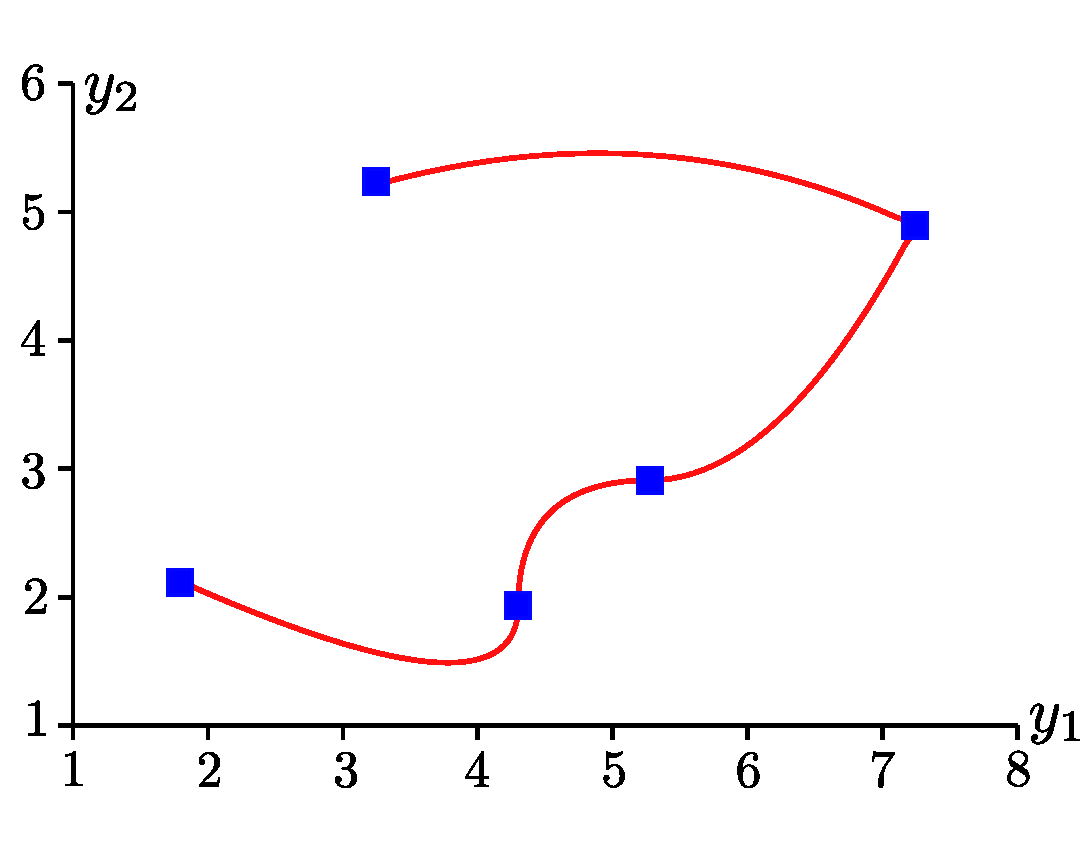
\includegraphics[scale=0.4,trim=0cm 0.7cm 0cm 0cm, clip=true]{Imagens/Cap3/bspline_curva.pdf}}
	\caption{Curva \textit{B-Spline}}
\end{figure}

A partir da Fig.\ref{fig:bspline_malhaPC} pode-se constatar que a curva \textit{B-Spline} interpola o primeiro e o último ponto de controle, que é uma característica das curvas construídas com funções descritas a partir de vetores de \textit{knots} abertos. Adicionalmente nota-se que, devido à multiplicidade do \textit{knot} de coordenada paramétrica $\xsi=3$, existe um ponto de controle intermediário também interpolando a curva. 
Coordenadas paramétricas com multiplicidade maior ou igual ao grau polinomial $p$ resultam, por definição, em interpolação dos pontos de controle associados.
Além disso, a curva possui continuidade $C^{p-1} = C^{1}$ em todos os lugares, exceto em $\xsi = 3$, onde equivale a $C^{p-2} = C^{0}$, que trata-se de uma propriedade herdada das funções base.

Conforme observado  Fig.\ref{fig:bspline_curva}, muitas das características de curvas \textit{B-Splines} são consequências das propriedades das funções \textit{B-splines}. Outra importante propriedade dessas curvas é a Transformação Afim, que significa que uma transformação afim de uma curva B-spline é obtida aplicando a transformação diretamente aos pontos de controle. Além disso, devido ao suporte compacto das funções base, as curvas \textit{B-Splines} possuem característica denominada de \textit{localidade}, que significa que, movendo-se um ponto de controle, afeta-se não mais do que $p+1$ células na curva. Outras propriedades matemáticas das curvas \textit{B-Splines} podem ser consultadas em detalhes em \citeonline{PiegT:1996}.

Uma superfície \textit{B-spline} é obtida analogamente à curva \textit{B-spline}. Dado uma rede de pontos de controle $\CP_{i,j}$ $\in \nrealspace$ com $i = 0,1,...,n$ e $j = 0,1,..., m$, e vetores de \textit{knots} $\Xsi = \left[\xsi_{0},\xsi_{1},...,\xsi_{p+n+1}\right]$, $\mathcal{H} = \left[\eta_{0},\eta_{1},...,\eta_{q+m+1}\right]$, a superfície é obtida através do produto tensorial entre $(n+1)$ funções univariadas $\Nb_{i,p}$ e $(m+1)$ funções univariadas $\Mb_{j,q}$ da seguinte forma:

\begin{align}
\mathbf{S} = \pos\left(\xsi,\eta\right)  = \sum_{i=0}^{n}\sum_{j=0}^{m}\Nb_{i,p}(\xsi)\Mb_{j,q}(\eta)\CP_{i,j},
\end{align}

\noindent onde $q$ representa o grau das $m+1$ funções na direção paramétrica $\eta$. 
Muitas das propriedades das superfícies \textit{B-Splines} são resultado da natureza do produto tensorial que as geram. A base de funções apresenta propriedade de positividade e formam uma partição de unidade, de forma que: $\forall(\xsi,\eta)$ $in \left[\xsi_{0},\xsi_{1},...,\xsi_{p+n+1}\right] \times  \left[\eta_{0},\eta_{1},...,\eta_{q+m+1}\right]$:

\begin{align}
 \sum_{i=0}^{n}\sum_{j=0}^{m}\Nb_{i,p}(\xsi)\Mb_{j,q}(\eta) = \left(\sum_{i=0}^{n} \Nb_{i,p}(\xsi)\right) \left(\sum_{j=0}^{m} \Mb_{j,q}(\eta)\right) = 1.
\end{align}

O suporte, por exemplo, de uma função bivariada $\hat{\Nb}_{i,j:p,q}\left(\xsi,\eta\right) = \Nb_{i,p}(\xsi)\Mb_{j,q}(\eta)$ é equivalente à: $\left[\xsi_{i},\xsi_{i+p+1}\right]\times\left[\eta_{j},\eta_{j+q+1}\right]$.

Por fim, um sólido \textit{B-Spline} é obtido através do produto tensorial entre funções univariadas $\Nb_{i,p}$, $\Mb_{j,q}$, $\Lb_{k,r}$, construídas sobre os vetores de \textit{knots} $\Xsi = \left[\xsi_{0},\xsi_{1},...,\xsi_{p+n+1}\right]$, $\mathcal{H} = \left[\eta_{0},\eta_{1},...,\eta_{q+m+1}\right]$ e $\mathcal{Z} = \left[\zeta_{0},\zeta_{1},...,\zeta_{r+l+1}\right]$ respectivamente, e um conjunto de pontos de controle  $\CP_{i,j,k}$ $\in \nrealspace$ com $i = 0,1,...,n$, $j = 0,1,..., m$, $k = 0,1,..., l$, da seguinte forma:

\begin{align}
\mathbf{T} = \pos\left(\xsi,\eta,\zeta\right)  = \sum_{i=0}^{n}\sum_{j=0}^{m}\sum_{k=0}^{l}\Nb_{i,p}(\xsi)\Mb_{j,q}(\eta)\Lb_{k,r}(\zeta)\CP_{i,j,k},
\end{align}

\noindent na qual $r$ representa o grau das $l+1$ funções base na direção paramétrica $\zeta$. As propriedades de um sólido \textit{B-Spline}, correspondem às generalizações trivariadas das propriedades das superfícies \textit{B-Spline}. Além disso, o suporte de uma função trivariada $\hat{\Nb}_{i,j,k:p,q,r}\left(\xsi,\eta,\zeta\right) = \Nb_{i,p}(\xsi)\Mb_{j,q}(\eta)\Lb_{k,r}(\zeta)$ está contido no intervalo $\left[\xsi_{i},\xsi_{i+p+1}\right]\times\left[\eta_{j},\eta_{j+q+1}\right]\times\left[\zeta_{k},\zeta_{k+r+1}\right]$.


\subsection{Refinamento}

Um dos aspectos mais relevantes das \textit{B-splines} é a flexibilidade na forma de enriquecimento da base, permitindo aprimorar sua representação sem alterar a geometria subjacente nem sua parametrização. Dentre os principais procedimentos utilizados, destacam-se: a inserção de \textit{knots} (ou refinamento $h$), que consiste na subdivisão da malha; a elevação de grau (ou refinamento $p$), que aumenta a ordem polinomial das funções base; o refinamento $k$, que promove simultaneamente um aumento da ordem e da continuidade entre células; e, por fim, o refinamento $hpk$, que combina de forma coordenada as três estratégias anteriores, oferecendo maior controle e eficiência na representação da geometria e na solução numérica de problemas.

Neste trabalho, será adotado na geração das geometrias o refinamento $h$, baseado na inserção de \textit{knots}. Por essa razão, somente essa estratégia será abordada ao longo desse texto.

O enriquecimento das funções base utilizando a inserção de \textit{knots} é realizado sem que se altere uma curva geometricamente ou parametricamente. Para essa finalidade, considerando o vetor de \textit{knots} $\Xsi = [\xsi_0,\xsi_1, ..., \xsi_{n+p+1}]$, será introduzido o conceito de vetor de \textit{knots} estendido, o qual compreende em: $\bar{\Xsi} = [\bar{\xsi}_0 = \xsi_0,\bar{\xsi}_1, ..., \bar{\xsi}_{n+m+p+1}= \xsi_{n+p+1}]$. As $(n+m+1)$ novas funções de base \textit{B-Splines} são determinadas através da Eq. \ref{eq:bsplines_0} e Eq. \ref{eq:bsplines_n}, aplicando-as ao vetor de \textit{knots} $\bar{\Xsi}$. Os $(n+m+1)$ novos pontos de controle  $\bar{\mathcal{B}} = [\bar{\CP}_0,\bar{\CP}_1,..., \bar{\CP}_{n+m}]^{T}$ são obtidos através da combinação linear dos $(n+1)$ pontos de controle originais, $\mathcal{B} = [\CP_0,\CP_1,..., \CP_{n}]^{T}$, por:


\begin{align}
	\bar{\mathcal{B}} = \mathbf{T}^{p}\mathcal{B},
\end{align}

\noindent, com:

\begin{align}
	\mathbf{T}_{ij}^{0} = \begin{cases} 1 &\mbox{se } \bar{\xsi}_i \in \left[\xsi_j,\xsi_{j+1}\right) \\
		0 & \mbox{caso contrário } \end{cases}, 
\end{align}

\begin{align}
	\mathbf{T}_{ij}^{q+1} = \frac{\bar{\xsi}_{i+q}-\xsi_j}{\xsi_{j+q}-\xsi_j}\mathbf{T}_{ij}^{q} + \frac{\xsi_{j+q+1}-\bar{\xsi}_{i+q}}{\xsi_{j+q+1}-\xsi_{j+1}}\mathbf{T}_{ij+1}^{q} \ \text{com} \ q=0,1,2,...,p-1,
\end{align}

\noindent sendo $i=0,1,...,(n+m)$ e $j=0,1,...,n$.

Considerando uma curva quadrática \textit{B-spline} construída sobre um vetor de \textit{knots} aberto $\Xsi=[0,0,0,1,1,1]$ apresentada na Fig. \ref{fig:bspline_pc_ai} juntamente com sua rede de pontos de controle. Essa curva, possui apenas uma célula no espaço físico, conforme pode ser observado na Fig. \ref{fig:bspline_curva_ai}, e $3$ funções base no espaço paramétrico (Fig. \ref{fig:bspline_base_ai}). Ao realizar-se a inserção de um \textit{knot}, $\xsi=1/2$, o vetor de \textit{knots} estendido fica definido como: $\bar{\Xsi}=[0,0,0,1/2,1,1,1]$. Aplicando-se as Eq. \ref{eq:bsplines_0} e Eq. \ref{eq:bsplines_n} à esse vetor de coordenadas paramétricas, obtém-se as $4$ funções base apresentadas na Fig.\ref{fig:bspline_base_di} definidas sobre 2 células do espaço paramétrico. Após o emprego do refinamento $h$, a geometria da curva é preservada. No entanto, como ilustrado na Fig. \ref{fig:bspline_curva_di}, uma nova célula física é inserida, além de que, de acordo com a Fig. \ref{fig:bspline_pc_di}, a malha de pontos de controle é modificada, com o acréscimo de um novo ponto e o reajuste de suas posições.


\begin{figure}[!t]
	\centering
	\subfloat[\label{fig:bspline_pc_ai}Curva original e pontos de pontrole]{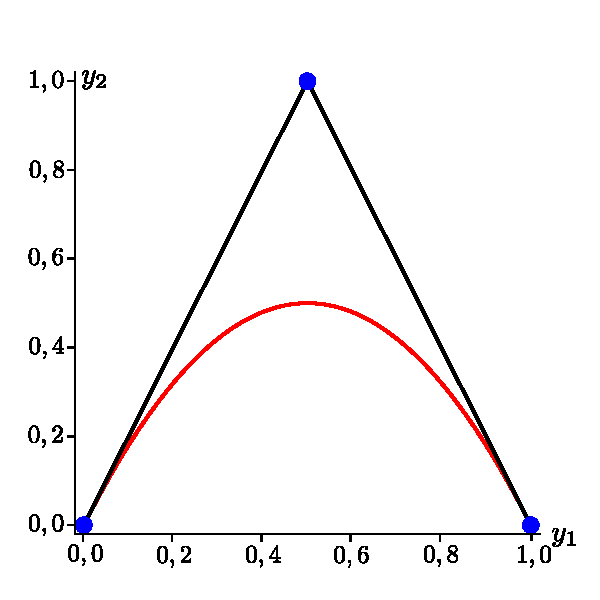
\includegraphics[scale=0.7,trim=0cm 0cm 0cm 1cm, clip=true]{Imagens/Cap3/bspline_pc_ai.pdf}} 
	\subfloat[\label{fig:bspline_pc_di}Curva refinada e pontos de controle]{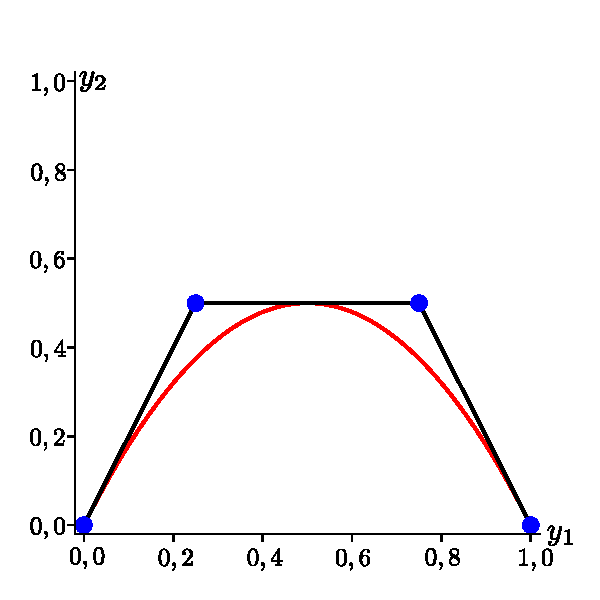
\includegraphics[scale=0.7,trim=0cm 0cm 0cm 1cm, clip=true]{Imagens/Cap3/bspline_pc_di.pdf}} \\ 
	\subfloat[\label{fig:bspline_curva_ai}Célula curva original]{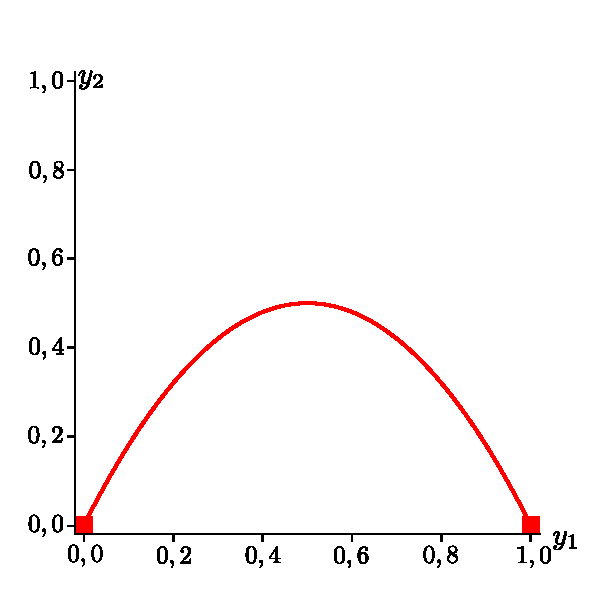
\includegraphics[scale=0.7,trim=0cm 0cm 0cm 1cm, clip=true]{Imagens/Cap3/bspline_curva_ai.pdf}} 
	\subfloat[\label{fig:bspline_curva_di}Células curva refinada]{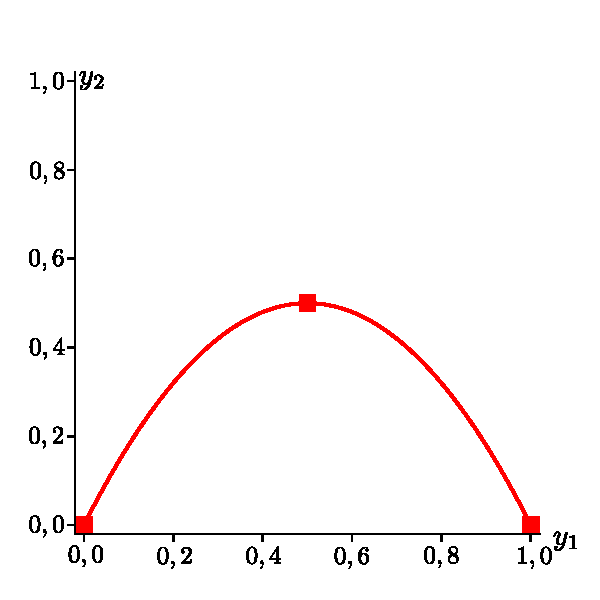
\includegraphics[scale=0.7,trim=0cm 0cm 0cm 1cm, clip=true]{Imagens/Cap3/bspline_curva_di.pdf}} \\ 
	\subfloat[\label{fig:bspline_base_ai}Funções base originais]{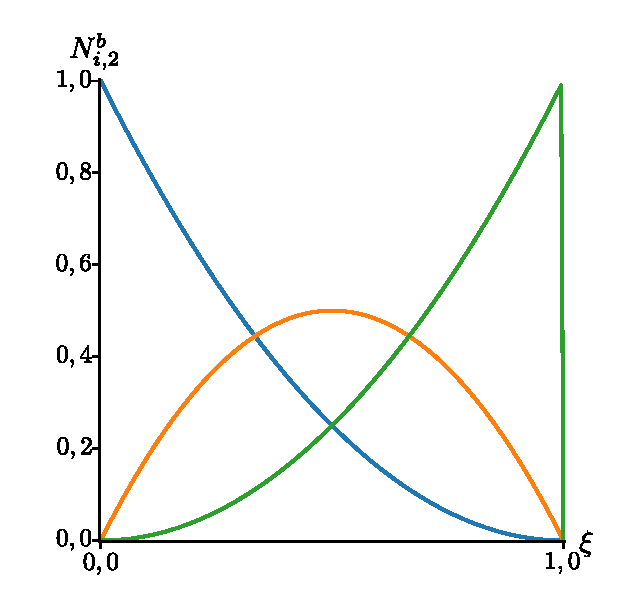
\includegraphics[scale=0.7,trim=0cm 0cm 0cm 0.5cm, clip=true]{Imagens/Cap3/bspline_base_ai.pdf}} 
	\subfloat[\label{fig:bspline_base_di}Funções base após refinamento $h$ refinada]{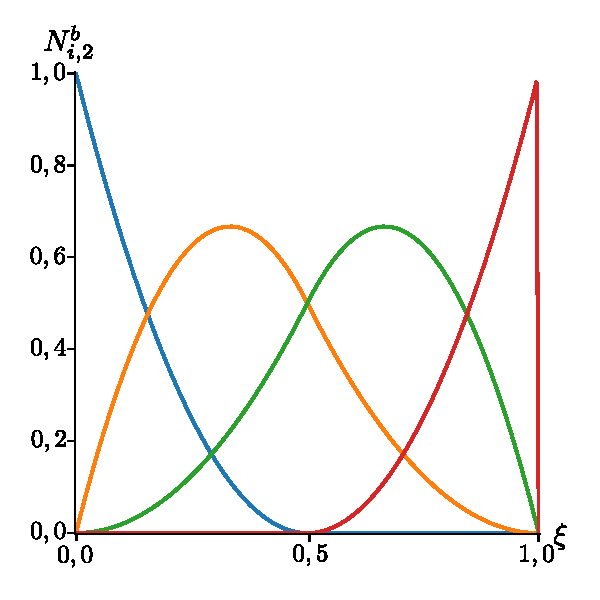
\includegraphics[scale=0.7,trim=0cm 0cm 0cm 0.4cm, clip=true]{Imagens/Cap3/bspline_base_di.pdf}} 
	\caption{Refinamento $h$ para um curva \textit{B-Spline}}
	\label{fig:bspline_insercaoKnots}
\end{figure}

Para fins práticos, o processo de refinamento consiste na inserção consecutiva de coordenadas paramétricas ao vetor de \textit(knots) até que se alcance a discretização desejada. Um algoritmo mais eficiente para realizar esse procedimento de refinamento pode ser encontrado em \citeonline{PiegT:1996}. Esse procedimento pode ser aplicado analogamente à superfícies e sólidos, aplicando-se a inserção de \textit{knots} nas direções paramétricas desejadas.


\section{NURBS}

Uma geometria NURBS no $\nrealspace$ pode ser entendida, do ponto de vista geométrico, como a transformação projetiva de uma geometria \textit{B-Spline} no $\realspace^{\nsd+1}$. Nesse contexto, geometrias cônicas podem ser construídas exatamente através de curvas quadráticas por partes. Na Fig. \ref{fig:NURBS_curva_transProj}, apresenta-se uma curva NURBS $\mathbf{C}\left(\xsi\right)$ no $\realspace^{2}$ , que representa de forma exata uma circunferência, a qual foi obtida a partir da transformação projetiva de uma curva quadrática por partes \textit{B-Spline} ($\mathbf{C}^{w}\left(\xsi\right)$) no  $\realspace^{3}$. A transformação é realizada através da projeção em um plano $y_3 = 1$ de cada ponto da curva projetiva ($\mathbf{C}^{w}\left(\xsi\right)$) através de um raio que passa pela origem.

\begin{figure}[!htb]
	\centering	
	\subfloat[Projeção transformativa malha de pontos de controle\label{fig:NURBS_PC_transProj}]{\includegraphics[scale=0.4,trim=0cm 0.0cm 0cm 0cm, clip=true]{Imagens/Cap3/NURBS_PC_projetiva.pdf}} \ \ 
	\subfloat[Projeção transformativa \textit{B-Spline} \label{fig:NURBS_curva_transProj}]{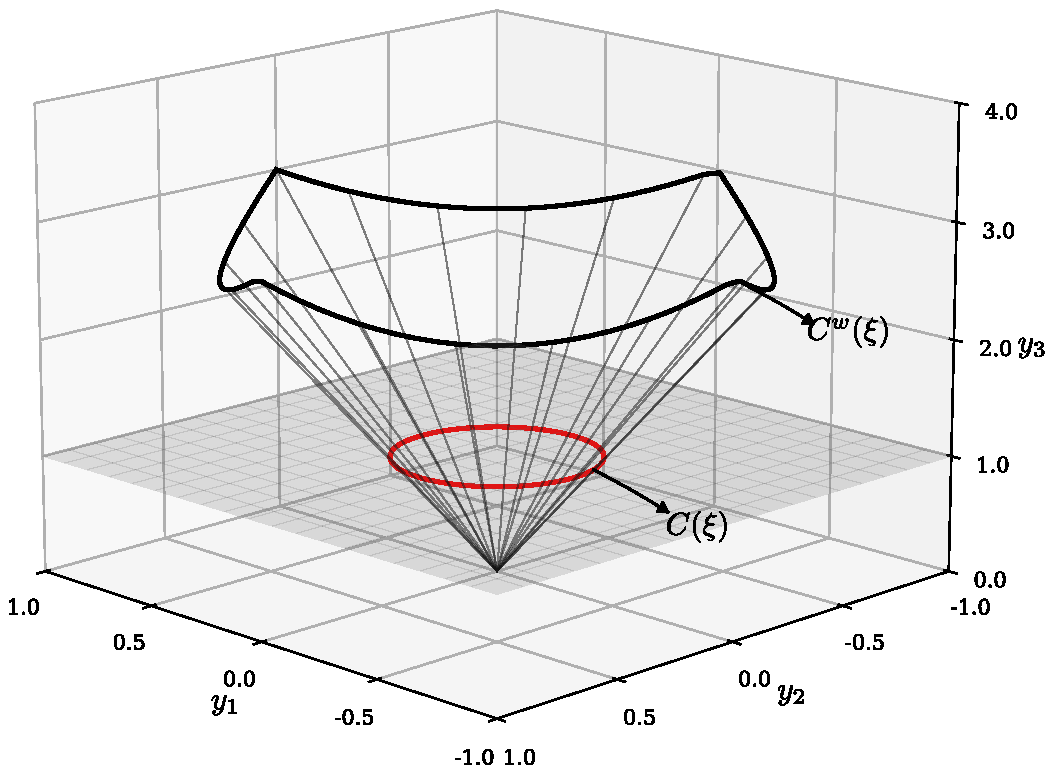
\includegraphics[scale=0.4,trim=0cm 0.0cm 0cm 0cm, clip=true]{Imagens/Cap3/NURBS_curva_projetiva.pdf}}
	\caption{Projeção transformativa de entidade \textit{B-Spline}}
\end{figure}

O mesmo procedimento de transformação pode ser realizado para obtenção dos pontos de controle NURBS (Fig. \ref{fig:NURBS_PC_transProj}) a partir de pontos de controle projetivos ($\mathbf{B_i}^w$), usando a seguinte relação:

\begin{align}
	\left(\CP_i\right)_j = \left(\CP^w_i\right)_j/w_i, \ \ j=1,...,\nsd ,
\end{align}

\begin{align}
	w_i =   \left(\CP^w_i\right)_{\nsd+1},
\end{align}

\noindent com $\left(\CP_i\right)_j$ o j-ésimo componente do vetor $\CP_i$ e $w_i$ refere-se ao i-ésimo peso, que consiste na coordenada $y_3$ dos pontos de controle projetivos para o exemplo citado.

Para a aplicação dessa mesma transformação para cada ponto da curva, será utilizado um conceito de função peso, dada por:

\begin{align}
	W(\xsi) = \sum_{\hat{i}=0}^{n}\Nb_{\hat{i},p}(\xsi)w_{\hat{i}},
\end{align}

e a curva NURBS pode ser definida como:

\begin{align}
	\left(\mathbf{C}(\xsi)\right)_j = \left(\mathbf{C}^w(\xsi)\right)_j/W(\xsi), \ \ j = 1,...,\nsd.
\end{align}

Tanto $\mathbf{C}^w$ como $W(\xsi)$ são funções polinomiais por partes, dessa forma, $\mathbf{C}(\xsi)$ é uma função racional por partes.

\subsection{Funções base NURBS e suas derivadas}

Matematicamente, uma função NURBS é obtida pela racionalização de uma função \textit{B-Spline}. A racionalização dessa função ocorre através da razão entre dois polinômios. Uma função racional NURBS $\left(\fNURBS\right)$ é construída através da seguinte expressão, dessa forma, têm-se:

\begin{align}
\fNURBS_{i,p}(\xsi) = \frac{\Nb_{i,p}(\xsi)w_i}{\sum_{\hat{i}=0}^{n}\Nb_{\hat{i},p}(\xsi)w_{\hat{i}}}.  \label{eq:NURBS_function}
\end{align}

\noindent com $w_{i}$ e $w_{\hat{i}}$ $\in \realspace$, sendo $i = \hat{i} =  0, 1, ... , n$.

A derivada de uma função $\fNURBS_{i,p}$ é obtida aplicando simplesmente a regra do quociente à expressão da Eq. \ref{eq:NURBS_function}:

\begin{align}
	\frac{\deriv}{\deriv \xsi} \fNURBS_{i,p}(\xsi) = w_{i} \frac{W\left(\xsi\right)\Nbl\left(\xsi\right) - W^{'}\left(\xsi\right)\Nb_{i,p}\left(\xsi\right)}{\left(W\left(\xsi\right)\right)^2},
\end{align}

\noindent com:

\begin{align}
	\Nbl\left(\xsi\right) \equiv \frac{\deriv}{\deriv \xsi} \Nb_{i,p}\left(\xsi\right),
\end{align}

\noindent e:

\begin{align}
	W^{'}\left(\xsi\right) = \sum_{\hat{i}=0}^{n} \Nblc \left(\xsi\right) w_{\hat{i}}.
\end{align}

A $k$-ésima derivada de $\fNURBS_{i,p}$ é obtida em termos de derivadas de menores ordem, através da seguinte expressão:

\begin{align}
\frac{\deriv^{k}}{\deriv \xsi^{k}} \fNURBS_{i,p}(\xsi) = \frac{A_{i}^{\left(k\right)} \left(\xsi\right) - \sum_{j=1}^{k} \binom{k}{j} W^{\left(j\right)} \left(\xsi\right) \frac{\deriv^{(k-j)}}{\deriv \xsi^{(k-j)}}\fNURBS_{i,p} \left(\xsi\right)}{W\left(\xsi\right)}
\end{align}

\noindent com:

\begin{align}
\binom{k}{j} = \frac{k!}{j!\left(k-j\right)!} ,
\end{align}

\begin{align}
	W^{\left(j\right)}\left(\xsi\right) = \frac{\deriv^{j}}{\deriv \xsi^{j}} W \left(\xsi\right) ,
\end{align}

\noindent e:

\begin{align}
 A_{i}^{\left(k\right)} \left(\xsi\right)  = w_i \frac{\deriv^k}{\deriv\xsi^k}\Nb_{i,p} \left(\xsi\right)\text{sem soma em $i$}.
\end{align}

\subsection{Geometria NURBS}

Uma curva NURBS é obtida através da combinação linear entre as funções base NURBS e um conjunto de pontos de controle, conforme expresso pela equação abaixo: 

\begin{align}
\mathbf{C} = \pos\left(\xsi\right) = \sum_{i=0}^{n}\fNURBS_{i,p}(\xsi)\CP_i, \label{eq:curveNURBS}
\end{align}

\noindent cujos pontos de controle e pesos são escolhidos criteriosamente de forma a obter-se a geometria desejada.

Analogamente uma superfície NURBS é obtida através das seguintes relações:

\begin{align}
\fNURBS_{i,j:p,q}(\xsi,\eta) = \frac{\Nb_{i,p}(\xsi)\Mb_{j,q}(\eta)w_{i,j}}{\sum_{\hat{i}=0}^{n}\sum_{\hat{j}=0}^{m}\Nb_{\hat{i},p}(\xsi)\Mb_{\hat{j},q}(\eta)w_{\hat{i},\hat{j}}},
\end{align}

\begin{align}
\mathbf{S} = \pos\left(\xsi,\eta\right) = \sum_{i=0}^{n}\sum_{j=0}^{m}\fNURBS_{i,j:p,q}(\xsi,\eta)\CP_{i,j}, \label{eq:surfaceNURBS}
\end{align}

\noindent com $w_{i,j}$ e $w_{\hat{i},\hat{j}}$ $\in \realspace$, sendo $i = \hat{i} =  0, 1, ... , n$ e  $j = \hat{j} =  0, 1, ... , m$ , correspondem aos pesos relativos às funções $\left(\Nb_{i,p}\left(\xsi\right)\Mb_{j,q}\left(\eta\right)\right)$ e $\left(\Nb_{\hat{i},p}\left(\xsi\right)\Mb_{\hat{j},q}\left(\eta\right)\right)$ respectivamente. Por fim, um sólido NURBS é obtido por:

\begin{align}
\fNURBS_{i,j,k:p,q,r}(\xsi,\eta,\zeta) = \frac{\Nb_{i,p}(\xsi)\Mb_{j,q}(\eta)\Lb_{k,r}(\zeta)w_{i,j,k}}
{\sum_{\hat{i}=0}^{n}\sum_{\hat{j}=0}^{m}\sum_{\hat{k}=0}^{l}\Nb_{\hat{i},p}(\xsi)\Mb_{\hat{j},q}(\eta)\Lb_{\hat{k},r}(\zeta)w_{\hat{i},\hat{j},\hat{k}}},
\end{align}

\begin{align}
\mathbf{T} = \pos\left(\xsi,\eta,\zeta\right) = \sum_{i=0}^{n}\sum_{j=0}^{m}\sum_{k=0}^{l}\fNURBS_{i,j,k:p,q,r}(\xsi,\eta,\zeta)\CP_{i,j,k}, \label{eq:solidNURBS}
\end{align}

\noindent onde $w_{i,j,k}$ e $w_{\hat{i},\hat{j},\hat{k}}$ $\in \realspace$, sendo $i = \hat{i} =  0, 1, ... , n$, $j = \hat{j} =  0, 1, ... , m$ e $k = \hat{k} =  0, 1, ... , l$, correspondem aos pesos relativos às funções $\left(\Nb_{i,p}\left(\xsi\right)\Mb_{j,q}\left(\eta\right)\Lb_{k,r}\left(\zeta\right)\right)$ e $(\Nb_{\hat{i},p}\left(\xsi\right)\Mb_{\hat{j},q}\left(\eta\right)\Lb_{\hat{k},r}\left(\zeta\right))$ respectivamente.

\subsection{Múltiplos \textit{Patches}}

Na grande maioria das situações práticas, é necessário para descrever um domínio computacional o uso de múltiplos \textit{Patches} NURBS, isto se deve ao fato que o produto tensorial do espaço paramétrico não é adequado para a representação de domínios complexos multiplamente conectados. Ademais, mesmo para domínios simples, do ponto de vista da simulação numérica, o uso de múltiplos \textit{patches} pode ser adequado para discretização das geometrias, conforme será visto na seção de exemplos.

\citeonline{HughesCB:2005} cita ainda que o uso de múltiplos \textit{patches} pode facilitar a análise numérica quando diferentes materiais e modelos físicos são utilizados em diferentes partes do domínio. E, além disso, em processamento paralelo, pode se tornar conveniente, do ponto de vista de estruturas de dados, não ter um único \textit{patch} entre diferentes processadores.

A utilização de múltiplos \textit{patches} implica na compatibilização da discretização na interface entre \textit{patches} adjacentes, ou seja, a parametrização e o mapeamento devem ser idênticos nesses locais. Cada ponto de controle em uma face de \textit{patches} adjacentes deve possuir um correspondente na outra face. Esses pontos iguais são tratados como um único ponto de controle dentro do sistema global resultante da análise numérica. 

Ressalta-se ainda, que na interface entre os \textit{patches}, devido a natureza interpolatória do vetores de \textit{knots} abertos, as funções base terão continuidade $C_0$, conforme pode ser observado na Fig. \ref{fig:multiplos_patches}, onde apresentam-se as funções base univariadas na interface entre dois \textit{patches}.

\begin{figure}[htb!]
	\centering 
	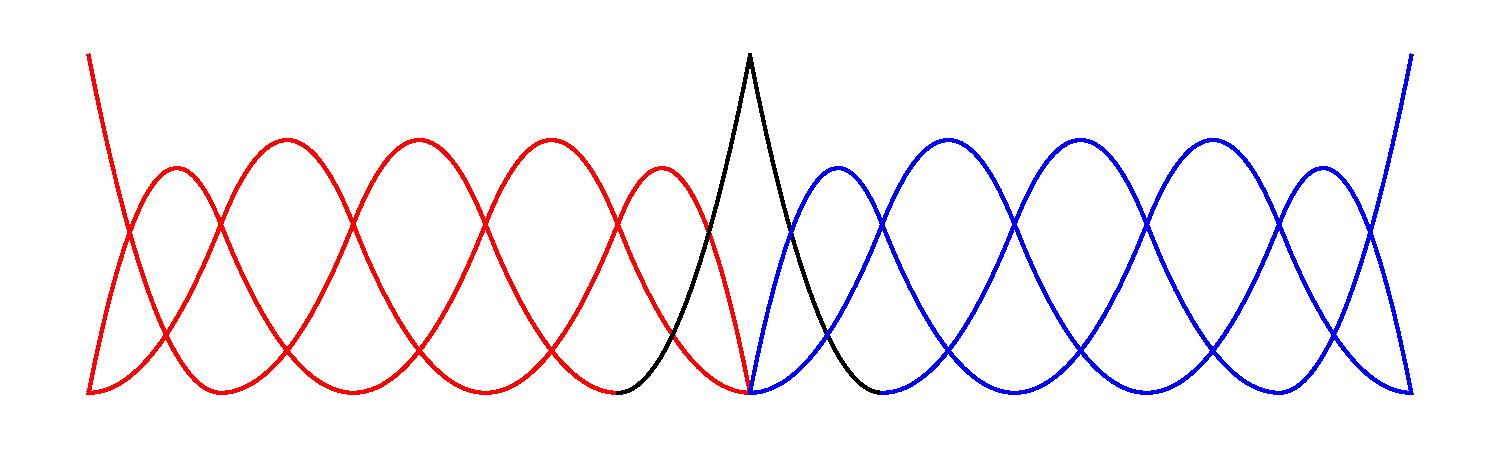
\includegraphics[scale=0.5,trim=0cm 0cm 0cm 0cm, clip=true]{Imagens/Cap3/patches.pdf}	
	\caption{Funções base univariadas na interface entre \textit{Patches}}
	\label{fig:multiplos_patches}
\end{figure}


\section{Análise Isogeométrica}


Para a aplicação da IGA no contexto da Dinâmica dos Fluidos Computacional, será utilizada como base a metodologia apresentada no Cap. \ref{capitulo:Cap2}. Nesse contexto, a aproximação da geometria, realizada no contexto do MEF pela Eq. \ref{eq:interp_geo}, será substituída pela abordagem Isogeométrica através do uso de geometrias NURBS, descritas pelas equações: Eq. \ref{eq:curveNURBS}, Eq. \ref{eq:surfaceNURBS} ou Eq. \ref{eq:solidNURBS} para os casos de curvas, superfícies ou sólidos respectivamente.

As funções tentativa para velocidade e pressão, e as funções teste associadas à elas, apresentadas nas Eq. \eqref{eq:interp_vel} à Eq. \eqref{eq:inter_ptest} como $N$, são equivalentes à $\fNURBS_{i,p}(\xsi)$, $\fNURBS_{i,j:p,q}(\xsi,\eta)$ e $\fNURBS_{i,j,k:p,q,r}(\xsi,\eta,\zeta)$ a depender da geometria em análise.

A integração numérica nas células é realizada através da quadratura Gaussiana. Considerando o domínio paramétrico de uma célula: $\bar{\domain}^{e}$, e o domínio de integração ou parental: $\tilde{\domain}^{e}$, apresentados na Fig.\ref{fig:espacos_NURBS}, definidos respectivamente pelos vetores de coordenadas paramétricas $\coordAdimen\left(\xsi,\eta,\zeta\right)$ e $\tilde{\coordAdimen}(\tilde{\xsi},\tilde{\eta},\tilde{\zeta})$, a matriz jacobiana do mapeamento do espaço físico, com coordenadas $\pos \left(y_1,y_2,y_3\right)$,  para o espaço de quadratura, é definida por:

\begin{align}
\frac{d\pos}{d\tilde{\coordAdimen}} = \frac{d\pos}{d\coordAdimen} \frac{d\coordAdimen}{d\tilde{\coordAdimen}}, \label{eq:integ}
\end{align} 

\noindent com $\tilde{\xi}, \tilde{\eta}, \tilde{\zeta} \in [-1, 1]$.

O primeiro termo à direita da igualdade da Eq. \eqref{eq:integ} é calculado a partir das derivadas parciais da Equação: Eq. \eqref{eq:curveNURBS}, Eq. \eqref{eq:surfaceNURBS} ou Eq. \eqref{eq:solidNURBS}, a depender do tipo da geometria em questão (curva, superfície ou sólido, respectivamente).

Para a obtenção do segundo termo à direita, primeiramente é necessário definir-se a relação entre as coordenadas  do domínio paramétrico e do domínio parental. Considerando-se a célula $\bar{\domain}^{e} = [\xsi_{i},\xsi_{i+1}] \times [\eta_{j},\eta_{j+1}] \times [\zeta_{k},\zeta_{k+1}]$, pode-se calcular $\xsi,\eta, \zeta$ $\in \bar{\domain}^{e}$ a partir de $\tilde{\xsi},\tilde{\eta}, \tilde{\zeta}$ $\in \tilde{\domain}^{e}$ através das seguintes relações: 

\begin{align}
\xsi = \xsi_{i} + \left(\tilde{\xsi}+1\right) \left(\frac{\xsi_{i+1}-\xsi_{i}}{2}\right), \label{eq:derXsi}
\end{align}

\begin{align}
\eta = \eta_{i} + \left(\tilde{\eta}+1\right) \left(\frac{\eta_{i+1}-\eta_{i}}{2}\right), \label{eq:derNeta}
\end{align}

\noindent e

\begin{align}
\zeta = \zeta_{i} + \left(\tilde{\zeta}+1\right) \left(\frac{\zeta_{i+1}-\zeta_{i}}{2}\right), \label{eq:derZeta}
\end{align}

\noindent assim, $\frac{d\coordAdimen}{d\tilde{\coordAdimen}}$ é obtido derivando-se parcialmente às expressões apresentadas em: Eq. \ref{eq:derXsi}, Eq. \ref{eq:derNeta} e Eq. \ref{eq:derZeta}.


\subsection{Parâmetros de estabilização}\label{capitulo:Cap3:RepreGeo:taus2}

Para a determinação dos parâmetros de estabilização $\tau$, de acordo com o exposto na Subseção \ref{capitulo:Cap2:FormaFraca:taus}, faz-se necessário a determinação de um tensor métrico, $\matrixG$ (Eq. \ref{eq:tensor_metrico}), o qual depende da matriz jacobiana transformada, $\matrixQhat$, definida na Eq. \ref{eq:q_chap}.

Devido a diferença entre o espaço paramétrico utilizado na definição das funções de base e do espaço paramétrico de integração, definido aqui como espaço parental, a matriz $\matrixQ$ será reescrita como:

\begin{align}
	\matrixQ&=\left(\frac{\partial\pos}{\partial\tilde{\coordAdimen}}\right).
\end{align}

Para a obtenção de $\matrixQhat$, de acordo com a Eq. \ref{eq:q_chap}, define-se a matriz $\matrixD$ para análise isogeométrica, de acordo com o trabalho de \citeonline{OtoguroTT:2020}, como:

\begin{align}
	\matrixD&=\left(\frac{\partial\hat{\coordAdimen}}{\partial\tilde{\coordAdimen}}\right),
\end{align}

\noindent que representa a relação entre o espaço paramétrico de preferência, onde o comprimento efetivo do elemento deve ser medido, e o espaço de integração, onde são definidos os pontos de quadratura.

O espaço paramétrico de preferência, para problemas unidimensionais, é definido para cada elemento por meio de uma interpolação usando polinômios de Bernstein $B_{b}^{p}$ de ordem $p$:

\begin{align}
	\hat{\xsi} \left(\tilde{\xsi}\right) = \sum_{b=0}^{p} \hat{\xsi}_b B_{b}^{p}\left(\tilde{\xsi}\right),
\end{align}

\noindent com os pontos de controle de Bézier, $\hat{\xsi}_b$, definidos igualmente espaçados da seguinte maneira:

\begin{align}
	\hat{\xsi}_b = \frac{\Delta{\hat{\xsi}}}{p}b,
\end{align}

\noindent sendo $\Delta{\hat{\xsi}}$ o comprimento paramétrico do elemento de Bézier. 

Os pontos de controle correspondentes no espaço de integração são dados por:

\begin{align}
	\tilde{\xsi}_a = \frac{\Delta{\hat{\xsi}}}{p} \sum_{b=0}^{p}b\left\{\matrixCinv\right\}_{ba},
\end{align}

\noindent com $a=0,...,p$. $\matrixC$ consiste no operador de extração de Bézier, que relaciona as funções B-spline globais às funções de Bernstein locais, cuja obtenção, nesse trabalho, é realizada de acordo com o exposto em \citeonline{BordenSEH}.

O comprimento efetivo de elemento para $a = 1, ..., p$ pode ser calculado por:

\begin{align}
	\Delta{\tilde{\xsi}_a} &= \tilde{\xsi}_a - \tilde{\xsi}_{a-1} \\
		           &= \frac{\Delta{\hat{\xsi}}}{p} \sum_{b=0}^{p}b\left(\left\{\matrixCinv\right\}_{ba} - \left\{\matrixCinv\right\}_{ba-1}\right).
\end{align}


A partir disso pode-se definir o razão entre o comprimento do elemento de Bézier e o comprimento efetivo do elemento. Considerando um problema 1D, uma das proposta dos autores para $D$, utilizada nesse trabalho, chama-se \textit{RQD-MAX} e consiste em:


\begin{align}
	D&=\frac{\Delta\hat{\xsi}}{\min_{a=1,...,p} \Delta\tilde{\xsi_{a}}},
\end{align}

\noindent resultando em:

\begin{align}
	D&={p}\left(\min_{a=1,...,p} \sum_{b=0}^{p} b \left(\left\{\matrixCinv\right\}_{ba} - \left\{\matrixCinv\right\}_{ba-1}\right)\right)^{-1} \\
	  &={p}\max_{a=1,...,p}\left(\sum_{b=0}^{p} b \left(\left\{\matrixCinv\right\}_{ba} - \left\{\matrixCinv\right\}_{ba-1}\right)\right)^{-1}
\end{align}

Para múltiplas dimensões o coeficiente de transformação $D$ é obtido individualmente para cada uma das direções do espaço paramétrico, e os componentes da matriz de transformação $\matrixD$ são determinados como:

\begin{align}
	D_{ij} = D^{i} \delta_{ij},
\end{align}

\noindent $i,j = 1,...,n_{pd}$, sendo $n_{pd}$ a dimensão do espaço paramétrico.


{\color{red}VOLTAR AQUI!}.


\section{Verificação e aplicações}

Para aplicação da IGA em problemas da DFC seguiu-se o mesmo procedimento matemático descrito ao longo do Cap. \ref{capitulo:Cap1}, sendo que a implementação computacional seguiu o roteiro apresentado no Alg. \ref{alg:fluid_temporalIntegration}. Os exemplos escolhidos para a verificação do código computacional foram o escoamento sobre um cilindro 3D e o problema de escoamento sobre um canal com degrau utilizando células 3D. Os resultados obtidos são apresentados nas seções subsequentes.

\subsection {Escoamento sobre um cilindro - 3D}

Na geração da geometria NURBS, correspondente ao problema do escoamento sobre um cilindro, utilizou-se um código previamente desenvolvido pela estudante durante seu mestrado \cite{Tonon:2016}. Por tratar-se de uma geometria de pequena complexidade, pôde-se gerá-la com um único \textit{patch}, o qual é composto por um cubo com um cilindro inserido em seu centro.
O processo de geração da malha, simplificadamente, consiste em se escolher vetores de $knots$, pontos de controle, e pesos adequados para a descrição de tal geometria.

O código previamente desenvolvido, baseia-se na quantidade mínima de pontos de controle necessários para gerar uma circunferência completa (ver Fig. \ref{fig:pontosdecontroleInicias}). Para a obtenção exata de uma circunferência utilizam-se funções quadráticas e o vetor de \textit {knots} na direção paramétrica $\xsi$ inicial é composto por: $\xsi=\left[0,0,0,1/4,1/4,1/2,1/2,3/4,3/4,1,1,1\right]$. A posição dos pontos de controle da circunferência e seus respectivos pesos foram obtidos de acordo com \citeonline {PiegT:1996}. 

A obtenção da curva respectiva ao quadrado, que é descrita no espaço paramétrico correspondente a direção $\xsi$, é consequência das escolhas realizadas para gerar a circunferência, logo, a curva possui o mesmo vetor de \textit{knots} e funções quadráticas. Os pontos de controle para a formação do quadrado foram posicionados, no espaço físico, de forma a ser obtida a dimensão requerida à seção transversal quadrada que compõe a geometria do cubo, e de forma que os mesmos ficassem alinhados com os pontos de controle da circunferência na direção radial. Os pesos respectivos ao pontos de controle do retângulo são unitários. Na Fig. \ref{fig:pontosdecontroleInicias} pode-se observar a posição dos pontos de controle respectivos à circunferência e ao quadrado e as curvas resultantes desta discretização em linha vermelho pontilhado.

Na sequência o código realiza o procedimento de refinamento por inserção sucessiva de \textit{knots} no vetor de \textit{knots}. O algoritmo utilizado para este procedimento pode ser encontrado em \citeonline {PiegT:1996}. Na Fig. \ref{fig:pontosdecontroleInicias2} apresenta-se um exemplo de pontos de controle gerados após a inserção de um novo \textit{knot} no centro de cada \textit{knot span} do espaço paramétrico inicial. A quantidade de \textit{knots} a ser inserida depende da discretização necessária a análise numérica.

\begin{figure}[!htb]
	\centering	
	\subfloat[Pontos de controle inicias.\label{fig:pontosdecontroleInicias}]{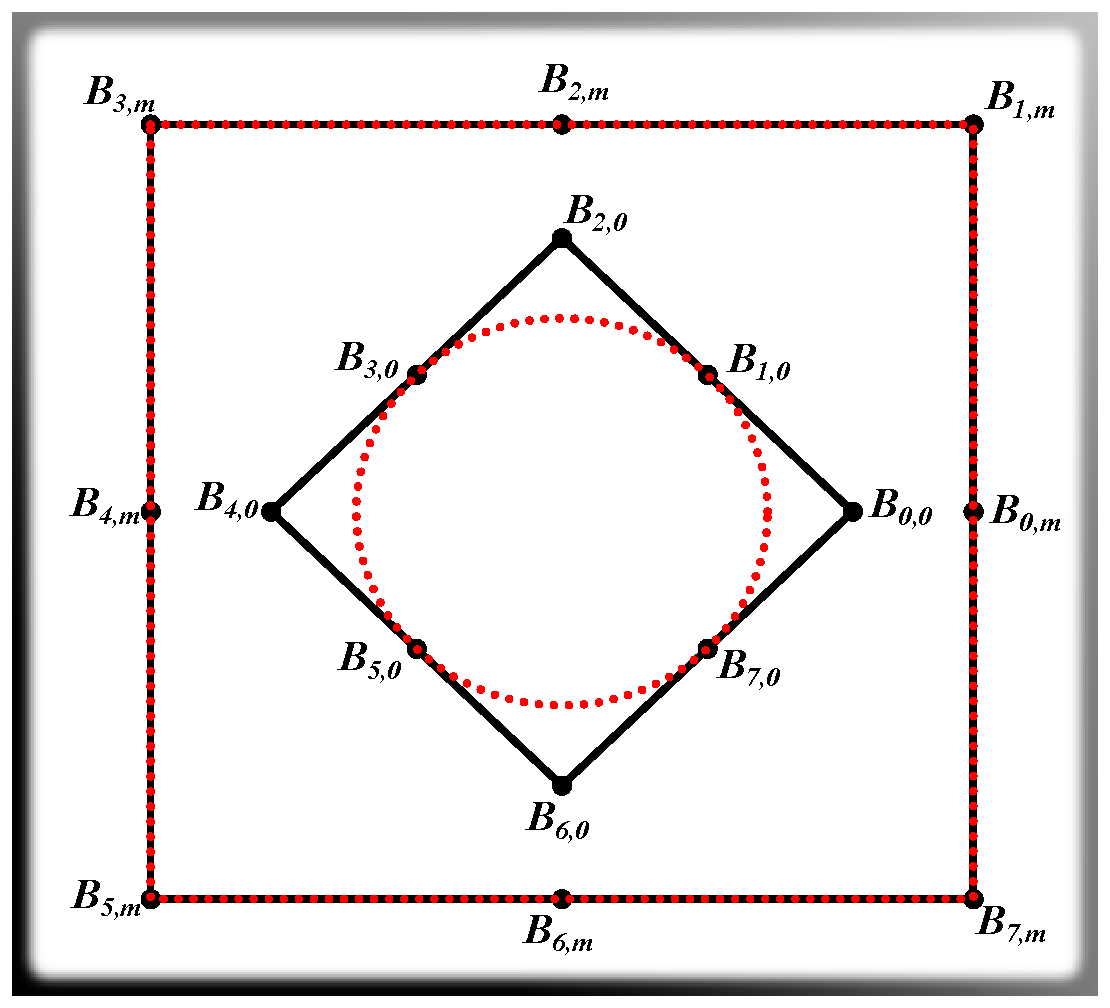
\includegraphics[scale=0.4,trim=1cm 1cm 0.5cm 1cm, clip=true]{Imagens/Cap3/escoamentosobrecilindro.pdf}}
	\subfloat[Pontos de controle após inserção de \textit{knots}.\label{fig:pontosdecontroleInicias2}]{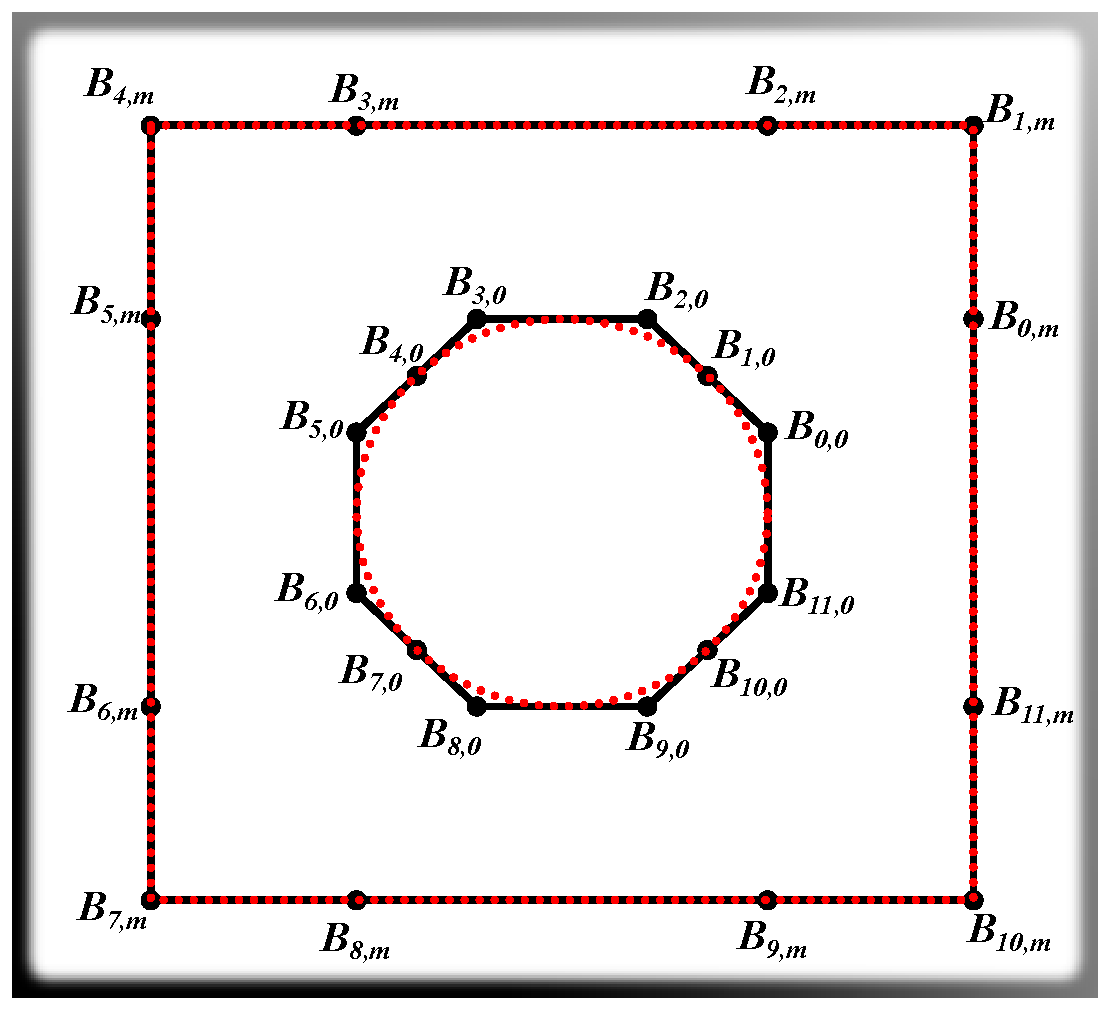
\includegraphics[trim=1cm 1cm 0.5cm 1cm,clip,scale=0.4]{Imagens/Cap3/escoamentosobrecilindro2.pdf}}
	\caption{Cilindro 3D: Geração curva NURBS}
\end{figure}

Para a obtenção de uma seção transversal da geometria em questão, gera-se uma superfície a partir da discretização na direção $\eta$ do espaço paramétrico. O código utiliza um vetor de \textit{knots} aberto, com os 
\textit{knots} distribuídos uniformemente, e funções de forma quadráticas. Os pontos de controle são distribuídos radialmente no espaço físico através de uma progressão geométrica unidirecional e seus pesos são determinados a partir de uma interpolação linear entre os pesos dos pontos de controle da circunferência e os pontos do quadrado. A quantidade mínima de pontos de controle respectiva à direção $\eta$ é de $q+1$ pontos, sendo a quantidade final definida em função da análise numérica. Na Fig. \ref{fig:superficieNURBcilindro}, apresenta-se um exemplo de uma rede de pontos de controle, obtida a partir das curvas apresentadas em Fig. \ref {fig:pontosdecontroleInicias2} com 9 pontos de controle na direção $\eta$. Na figura em questão omitiu-se a nomenclatura dos pontos de controle intermediários às curvas da circunferência e do quadrado para evitar a sobreposição da nomenclatura na figura.


\begin{figure}[htb!]
	\centering 
	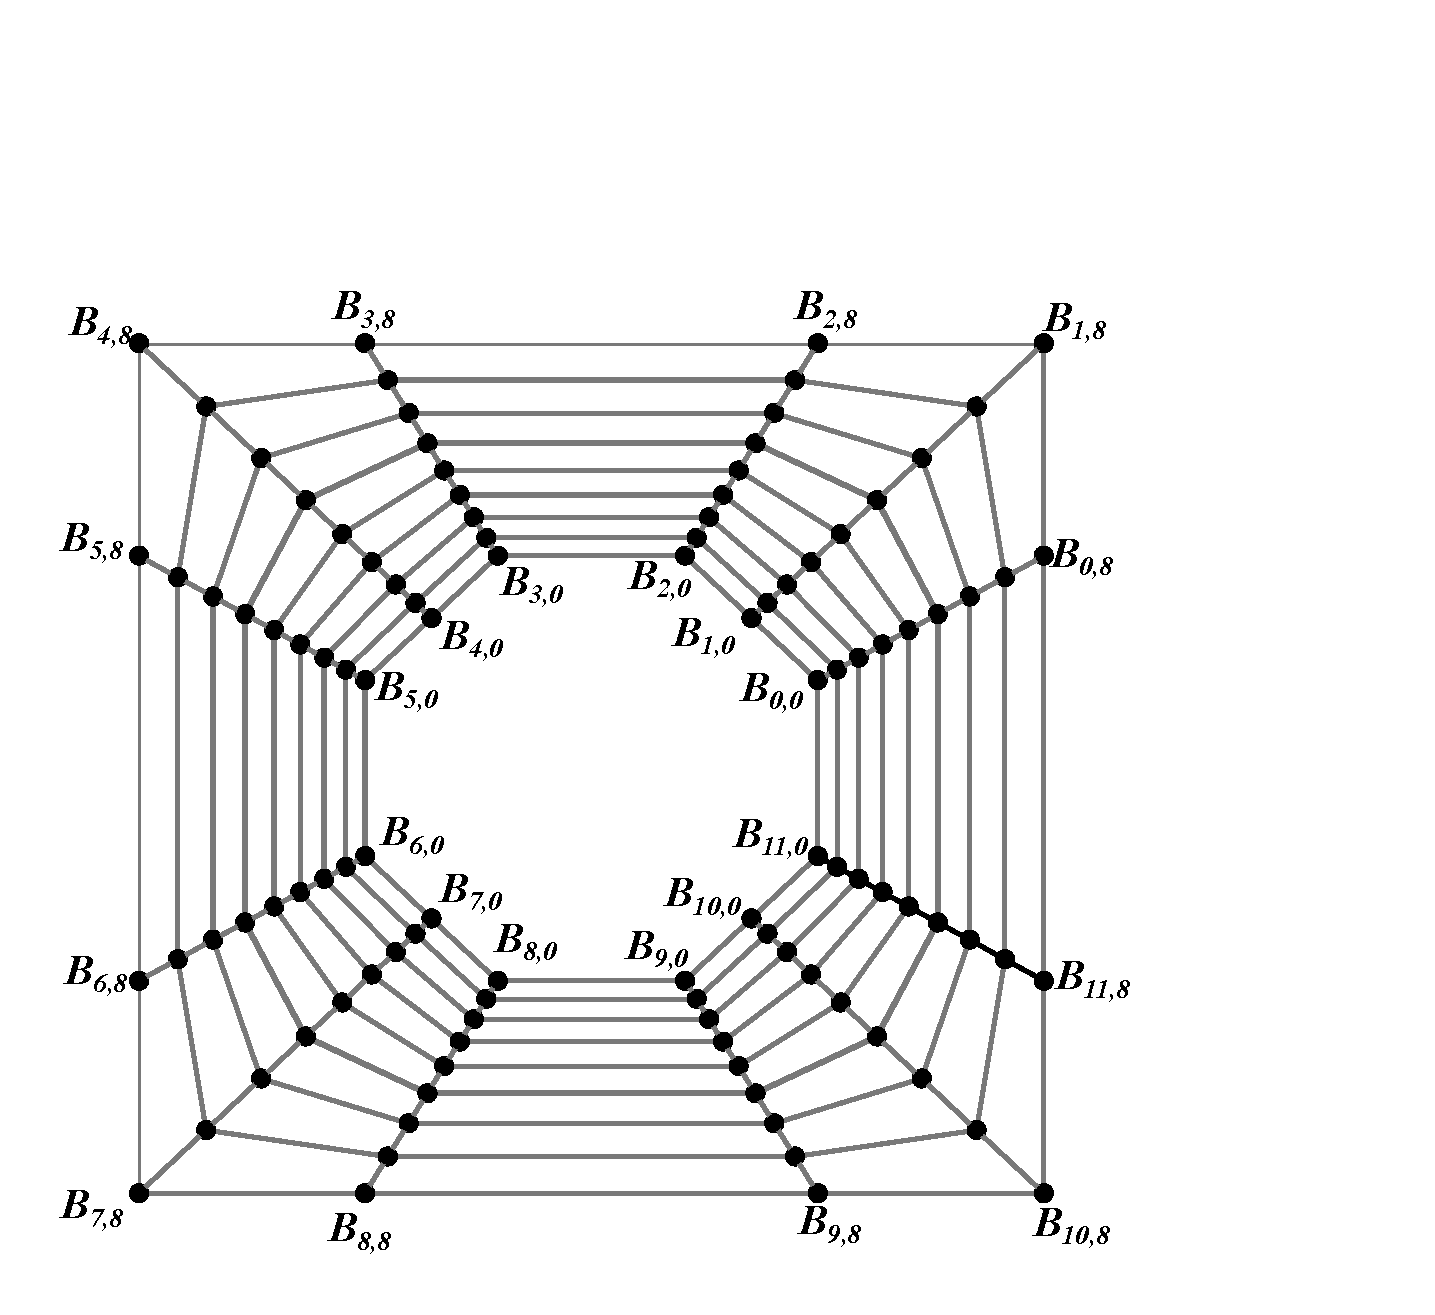
\includegraphics[scale=0.4,trim=1cm 1cm 5cm 4cm, clip=true]{Imagens/Cap3/escoamentosobrecilindro3.pdf}	
	\label{fig:superficieNURBcilindro}
	\caption{Cilindro 3D: Geração superfície NURBS.}
\end{figure}

Nessa primeira etapa do trabalho, a direção paramétrica $\zeta$, respectiva à direção $z$ da geometria física, foi discretizada com apenas uma célula, utilizando-se para isso vetor de \textit{knots} abertos com distribuição uniforme de \textit{knots}, e funções base quadráticas.

Visando a verificação do código de IGA 3D analisa-se o problema do escoamento sobre o cilindro para $\Reynolds$ =40 ,100 e 1000 (Eq. \eqref{eq:Reynolds}). Para isso, gera-se uma malha com 101 x 71 x 3 pontos de controle nas direções paramétricas $\xsi$, $\eta$ e $\zeta$ respectivamente, resultando em 6624 células. Na Fig. \ref{fig:cilindrogeometria} apresentam-se as dimensões da geometria em questão, bem como as condições de contorno aplicadas, e na Fig. \ref{fig:cilindromalha} apresenta-se a malha física resultante da discretização.


\begin{figure}[!htb]
	\centering
	\subfloat[\label{fig:cilindrogeometria}Geometria]{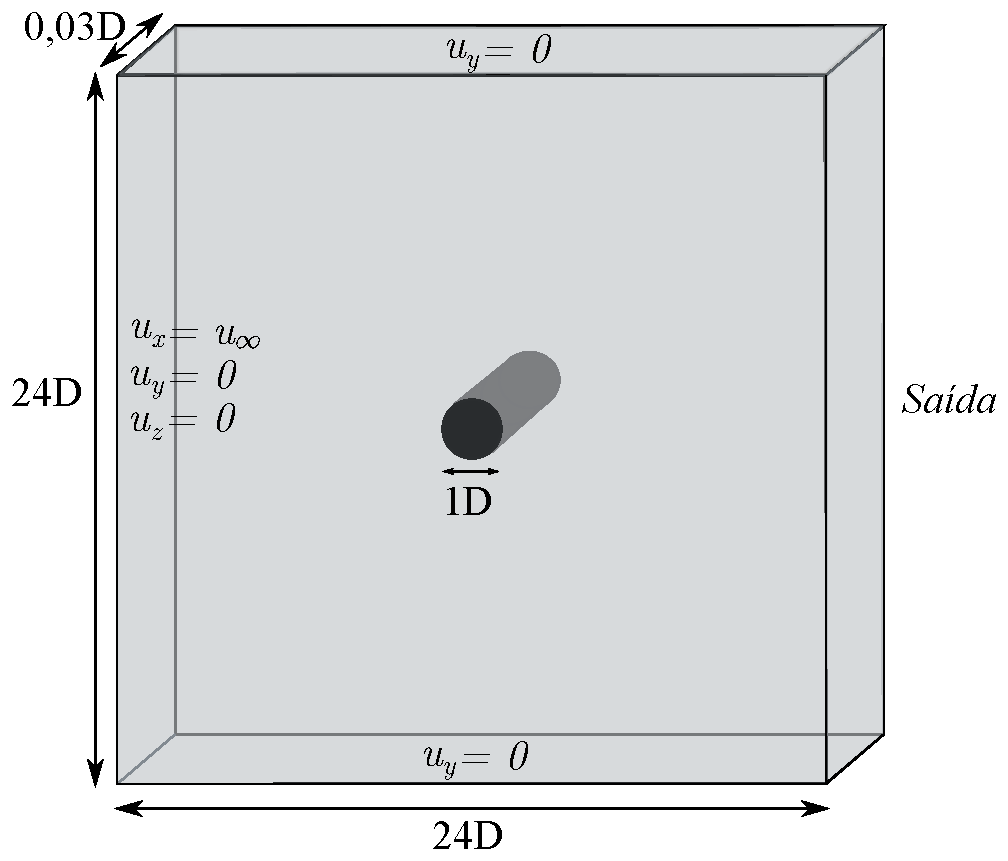
\includegraphics[scale=0.48,trim=0cm 0cm 0cm 0cm, clip=true]{Imagens/Cap3/cylinderISO3d.pdf}} 
	\subfloat[\label{fig:cilindromalha} Malha de células físicas]{\includegraphics[scale=0.2,trim=5cm 0cm 0cm 0cm, clip=true]{Imagens/Cap3/malhacilindro.eps}} 
	\caption{Cilindro 3D: Geometria e malha de células físicas}
	\label{fig:cilindro_geoemalha}
\end{figure}

Adicionalmente, prescrevem-se nas paredes frontal e posterior, condição de parede lisa ($u_{z} = 0$), e na \textit{Saída} do escoamento condição de força de superfície nula ($\stressTensor \normal = \mathbf{0}$). O problema é simulado para um velocidade de entrada $u_{\infty} = 1,0$, $\rho = 1,0$, $\timeStep = 0,05$, e $\specRadius = 0,5$, sendo a viscosidade variada de acordo com o número de Reynolds desejado.  Para o cálculo dos coeficientes aerodinâmicos $C_{D}$, $C_{L}$ e do número de Strouhal ($\Strouhal$) utilizam-se as equações apresentadas no Item \ref{subsection:escoamentocil2d}. 

Nas Figs. \ref{fig:cilindro_Cd3d} e \ref{fig:cilindro_Cl3d}, apresentam-se a variação ao longo do tempo dos coeficientes $C_{D}$ e $C_{L}$. Os valores obtidos com a malha isogeométrica 3D estão muito próximos ao obtidos com a malha de elementos finitos 2D (Item \ref{subsection:escoamentocil2d}) para Reynolds 40 e 100. Para Reynolds 1000, nota-se que a variação ao longo do tempo dos valores de $C_{D}$ e $C_{L}$ para IGA resulta em valores mais elevados do que os obtidos com MEF. Tal diferença ainda deverá ser investigada, sendo que tanto as diferenças nas dimensões das malhas como a diferença que pode haver na convergência dos resultados ou a efeitos de 3D de vorticidade podem contribuir para isso. Os resultados obtidos para o histórico de $C_{D}$ e $C_{L}$ por \citeonline{Henderson:1997} para $Re = 1000$ em análises tridimensionais baseadas em MEF, foram menores do que os 2D. Essa disparidade entre os resultados obtidos nesse trabalho e de \citeonline{Henderson:1997} podem estar relacionados com o fato de que a dimensão escolhida da malha na direção $z$ foi muito pequena de maneira a impossibilitar que os efeitos tridimensionais do escoamento fossem adequadamente capturados.

Para o número de Strouhal, o valor obtido para $\Reynolds = 100$ foi de 0,1681 e para $\Reynolds = 1000$ de 0,2395. Nota-se que, embora os valores de $C_{D}$ e $C_{L}$ apresentem diferenças entre os resultados 2d baseados em elementos finitos e a malha 3D baseada em IGA, a frequência do desprendimento de vórtices obtida foi muito semelhante.

\begin{figure}[!htb]
	\centering
	\subfloat[\label{fig:cilindro_Cd3d}Coeficiente de arrasto $ C_D$.]{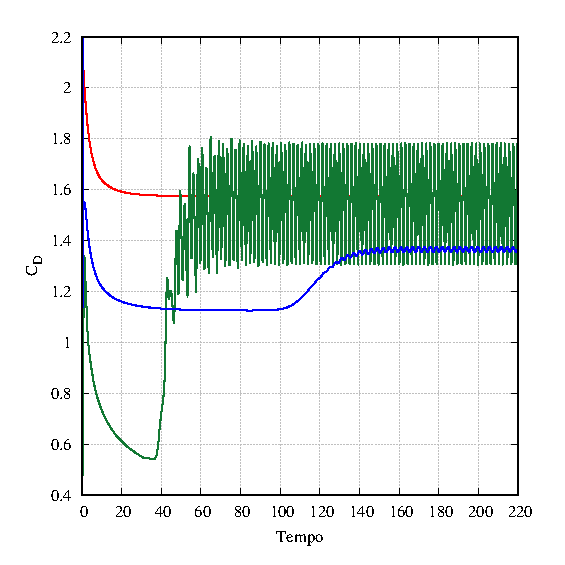
\includegraphics[scale=0.8,trim=0cm 0cm 0cm 0cm, clip=true]{Imagens/Cap3/DragRe.eps}} 
	\subfloat[\label{fig:cilindro_Cl3d}Coeficiente de sustentação $C_L$.]{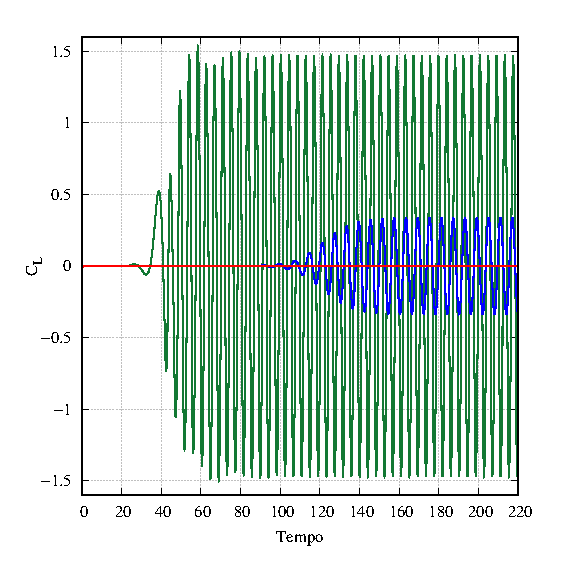
\includegraphics[scale=0.8,trim=0cm 0cm 0cm 0cm, clip=true]{Imagens/Cap3/LiftRe.eps}}\\ 
	{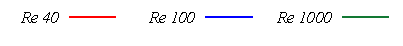
\includegraphics[scale=1.3]{Imagens/Cap3/Legenda.pdf}}
	\caption{Cilindro 3D: Coeficientes aerodinâmicos. }
	\label{fig:cilindro_coeficientes3d}
\end{figure}


\subsection {Escoamento em um canal com degrau}

Este exemplo é amplamento utilizado na verificação de códigos para escoamentos incompressíveis, sendo sua geometria apresentada na Fig. \ref{fig:degrau_geo}.  O problema consiste em prescrever-se um perfil parabólico de escoamento na entrada do canal, e condição de aderência ($\velocity = 0$) nas demais paredes que estão contidas nos planos $xz$ e $yz$, exceto na saída do canal, a qual possui como condição $\stressTensor\normal = \mathbf{0}$. Para as paredes dos planos $xy$, frontal e posterior, prescreveu-se condição de parede lisa ($u_{z}=0$). 

\begin{figure}[htb!]
	\centering
	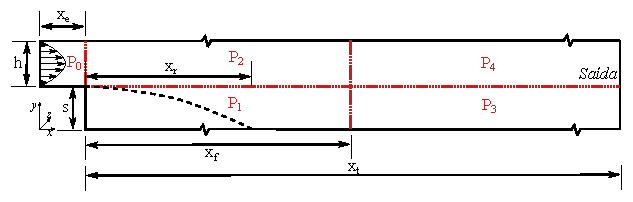
\includegraphics[scale=1.2,trim=0cm 0cm 0cm 0cm, clip=true]{Imagens/Cap3/degrau.pdf}
	\caption{Degrau 3D: Geometria.}
	\label{fig:degrau_geo}
\end{figure}


As dimensões selecionadas para o canal foram $h = 1,0m$, $s = 0,94m$, $x_{e}= 1,0m$, $x_{f}= 15m$ e $x_{t} = 30m$ e dimensão na direção $z$ de $0,1m$. Adicionalmente, o perfil de velocidade na entrada do canal é descrito pela seguinte relação:

\begin{align}
u_{x} = V_{max} \left(1-\left(\frac{\left(y-s\right)-h/2}{h/2}\right)^{2}\right),
\end{align}

\noindent com velocidade $V_{max} = 10 m/s$ e $u_{y} = u_{z} = 0$.

O escoamento sobre o degrau é caracterizado por produzir áreas de recirculação onde o fluido se separa e forma vórtices. A distância entre o degrau e o ponto de recolamento do vórtice principal $x_{r}$ é uma das principais características verificadas nesse problema. A dimensão dos vórtices varia em função do número de $\Reynolds$, a qual é calculada de acordo com \citeonline {ArmalyDP:1983}, sendo expressa por:

\begin{align}
\Reynolds =\frac{\rho\left(\frac{2V_{max}}{3}\right)2h}{\viscosity},
\end{align}

\noindent com $\rho = 1kg/m^{3}$. Foram selecionados para as análises 3 diferentes número de Reynolds: $100$, $400$ e $800$, variando-se a viscosidade do fluido.

Para a geração da geometria NURBS, discretiza-se o canal em 5 \textit{patches}, os quais são denominados $P_{0},P_{1},P_{2},P_{3}$ e $P_{4}$, e podem ser observados na Fig. \ref{fig:degrau_geo}. Todas as direções paramétricas são discretizadas com vetores de \textit{knots} abertos e com \textit{knots} igualmente espaçados no interior do vetor, além de funções de forma quadráticas. Os pontos de controle para os \textit{patches} $0,1$ e $2$ foram distribuídos no espaço físico, direções $x,y$ e $z$ de maneira a se obter células igualmente espaçados. Para os \textit{patches} $3$ e $4$, na direção do espaço físico $y$ e $z$, os pontos são posicionadas de maneira a gerar células uniformes, e, na direção $x$, são distribuídos de maneira a se resultar numa progressão geométrica do tamanho das células, com as células aumentando de tamanho da esquerda para a direita, conforme pode ser observado na Fig. \ref{fig:degrau_malha}. Na Tab. \ref{tab:numberPCpatches} podem ser observados os números de pontos de controle utilizados em cada direção dos espaços paramétricos para cada \textit{patch}, resultando em 60795 pontos de controle e 4800 células.

\begin{figure}[htb!]
	\centering
	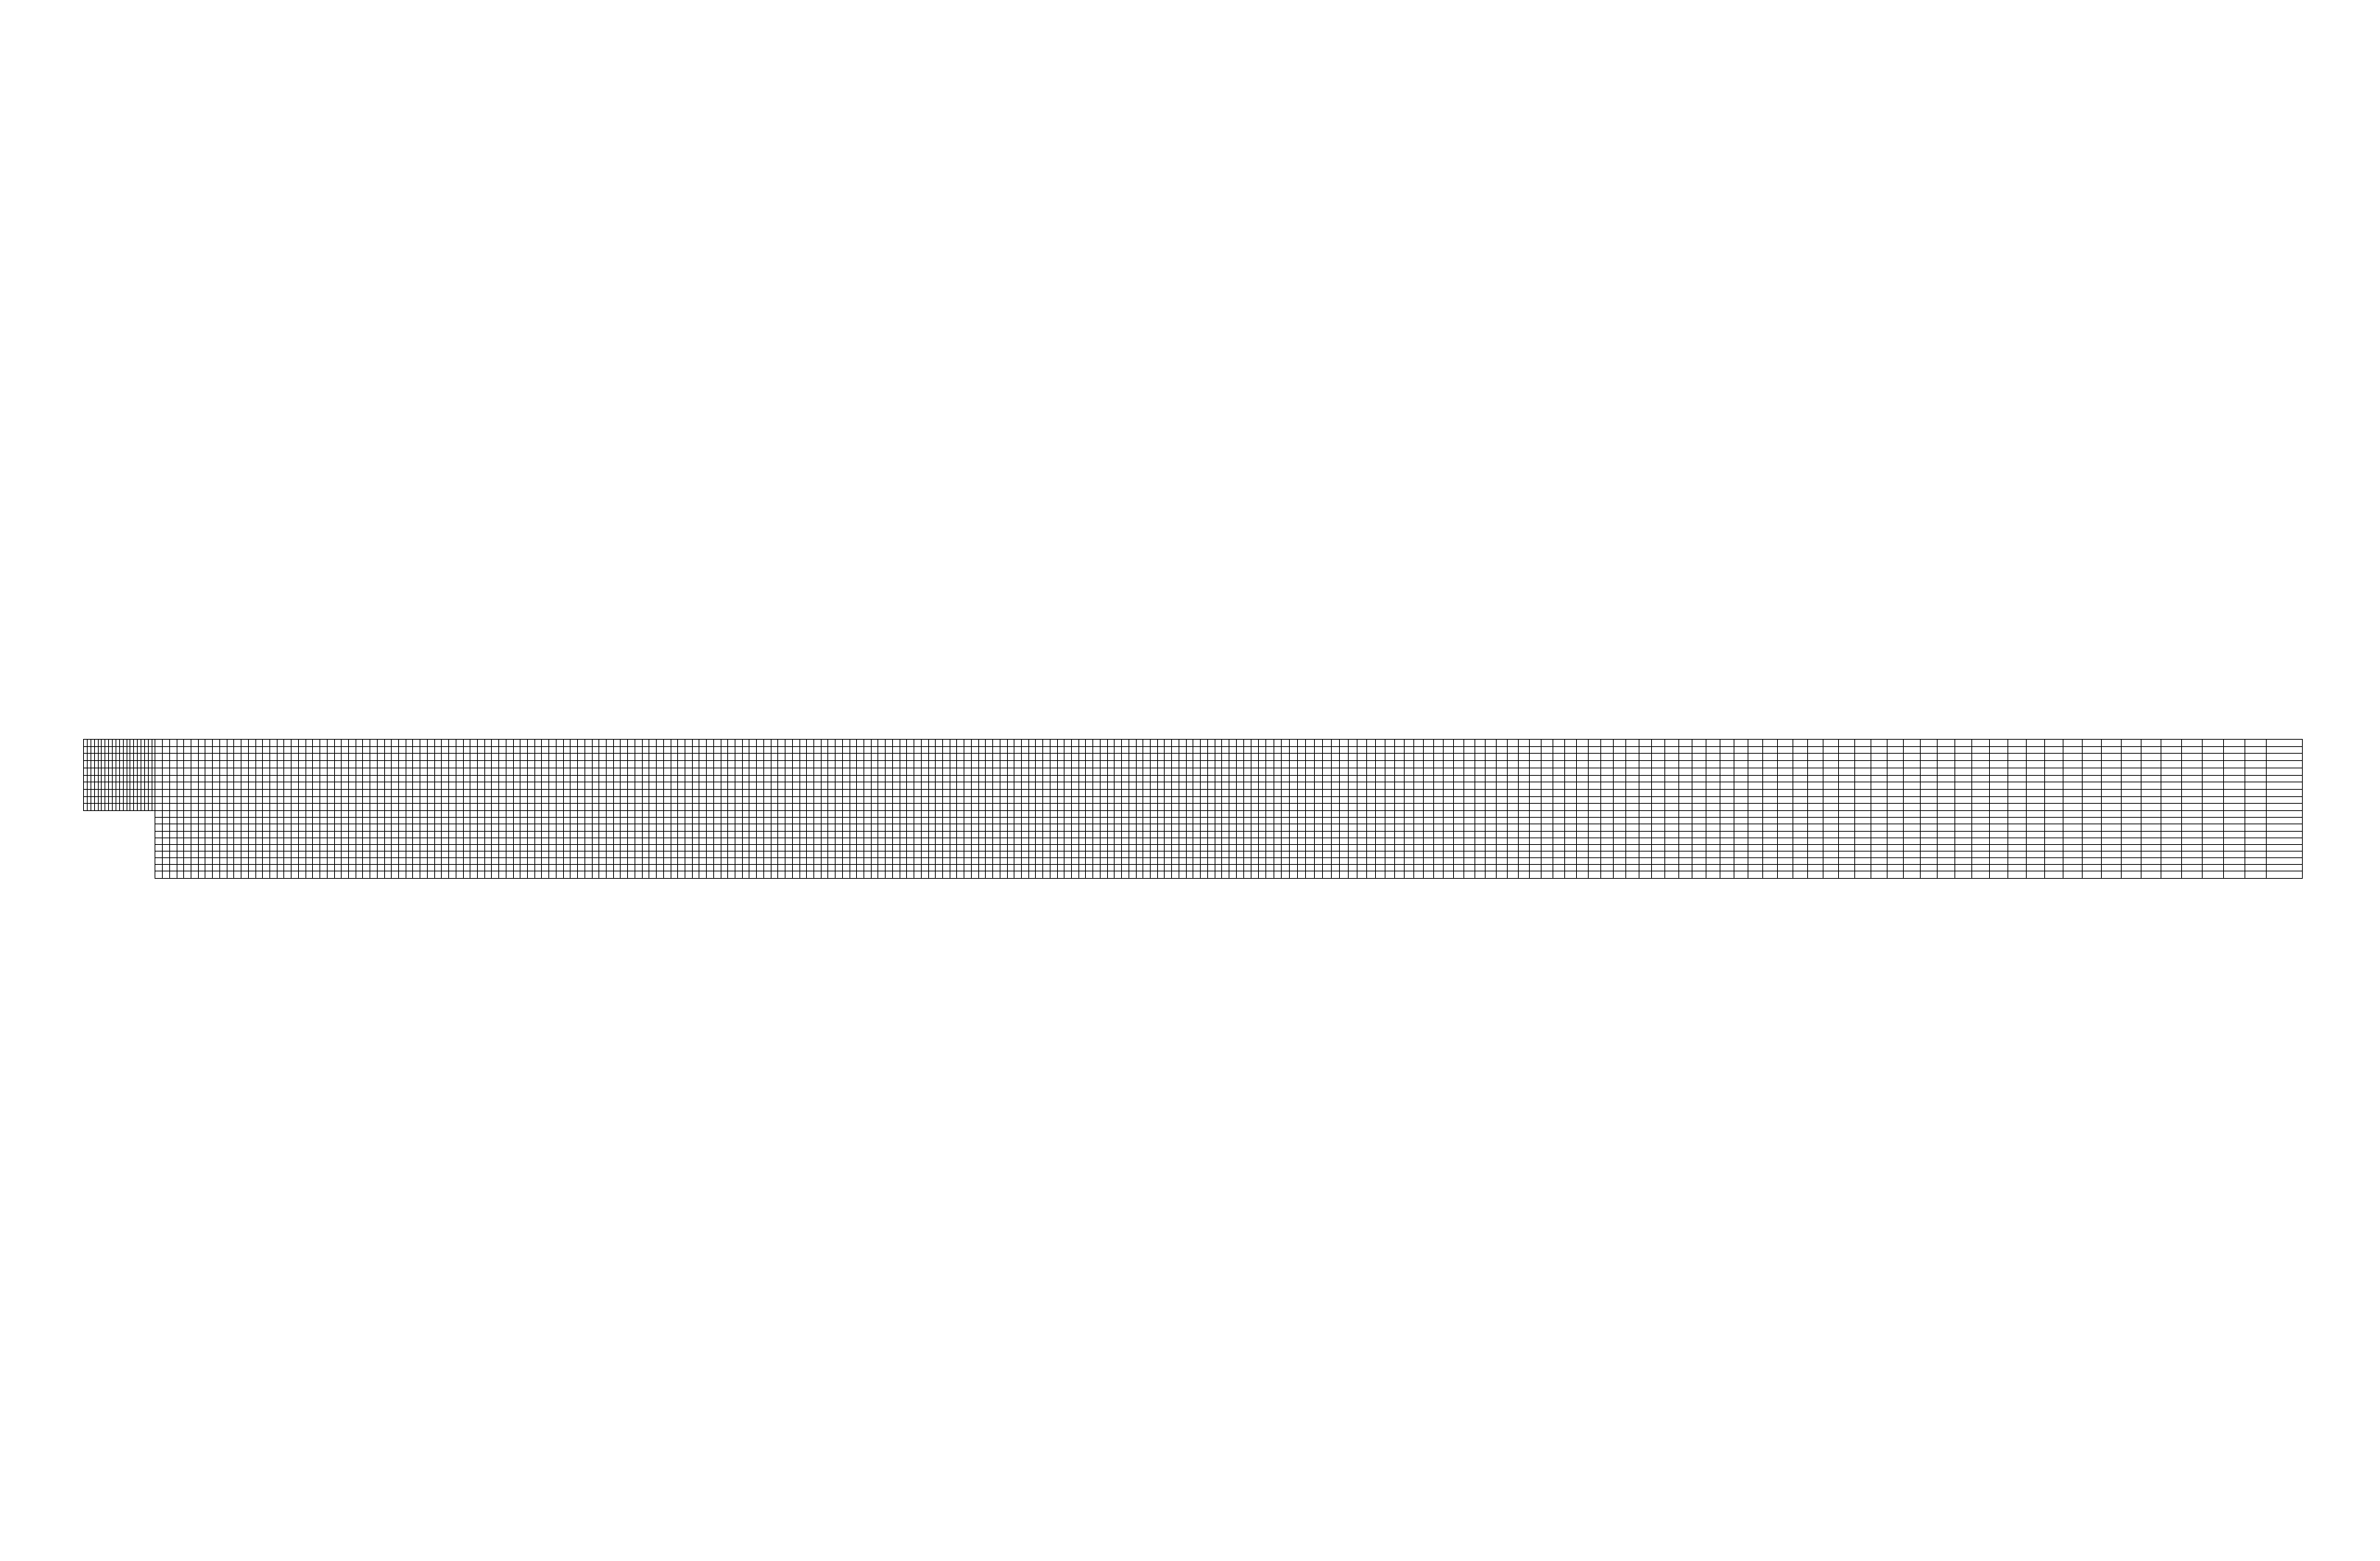
\includegraphics[scale=0.3,trim=1cm 14cm 1cm 14cm, clip=true]{Imagens/Cap3/malhadegrau.eps}
	\caption{Degrau 3D: Geometria e malha de células físicas}
	\label{fig:degrau_malha}
\end{figure}

\begin{center}
	\begin{table}[h!]
		\caption{Número de pontos de controle por \textit{patch}}
		\centering
		\begin{tabular}{|c | c | c| c|} 
			\hline
			\textit{Patch} & $\xsi$ & $\eta$ & $\zeta$ \\ 
			\hline
			0 & 22 & 12 & 3 \\ 
			\hline
			1 & 152 & 12 & 3\\
			\hline
			2 & 152 & 12 & 3\\
			\hline
			3 & 82 & 12 & 3\\
			\hline
			4 & 82 & 12 & 3\\
			\hline
		\end{tabular}
		\label{tab:numberPCpatches}
	\end{table}
\end{center}


Na Fig. \ref{fig:degrau_com_recl} são apresentados os comprimentos de recolamento do vórtice primário adimensionalizados ($x_{r}/s$), juntamente com os resultados adaptados dos ensaios experimentais de \citeonline{ArmalyDP:1983} e os resultados de análises 2d de \citeonline{WilliamsB:1999}. Nota-se que os resultados obtidos estão próximos das referências para $\Reynolds = 100$ e $\Reynolds =400$, entretanto, para $\Reynolds = 800$ nota-se um afastamento do presente trabalho, e do referente à análise 2D com relação ao experimento realizado por \citeonline{ArmalyDP:1983}. Isto ocorre, visto que o ensaio experimental foi realizado com um canal com $2m$ de comprimento na direção $z$, e a simulação atual com apenas uma célula nessa direção é incapaz de captar os fenômenos tridimensionais que ocorrem a medida que o número de Reynolds cresce. Na Fig.\ref {fig:degrau_vortices} pode-se observar o campo de velocidade para os Reynolds estudados, e o aspecto do vórtice primário desenvolvido.


\begin{figure}[htb!]
	\centering
	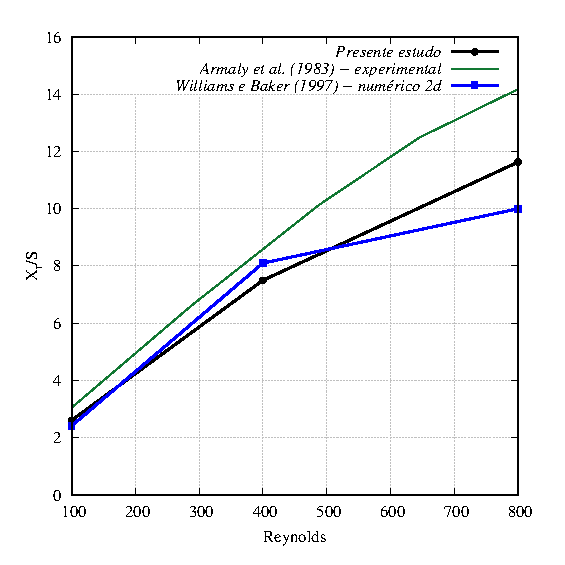
\includegraphics[scale=1.2,trim=0cm 0cm 0cm 0cm, clip=true]{Imagens/Cap3/comvort.eps}
	\caption{Degrau 3D: Comprimento de recolamento do v\'ortice principal}
	\label{fig:degrau_com_recl}
\end{figure}


\begin{figure}[!htb]
	\centering
	\subfloat[\label{fig:vortice_re100} $\Reynolds= 100$]{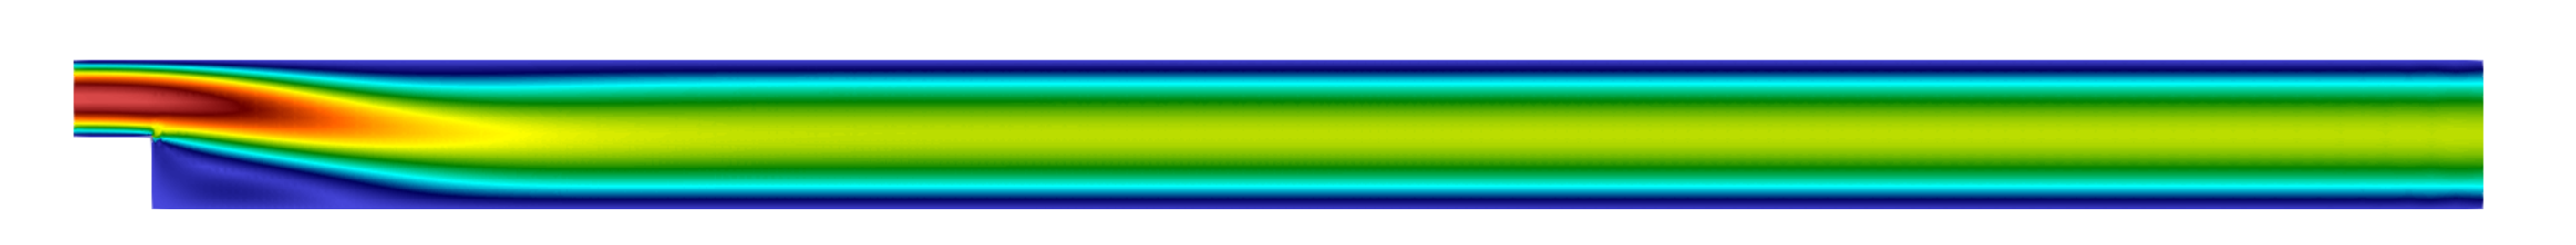
\includegraphics[scale=0.3,trim=0cm 0cm 0cm 0cm, clip=true]{Imagens/Cap3/degrau100.pdf}} \\
	\subfloat[\label{fig:vortice_re400} $\Reynolds= 400$]{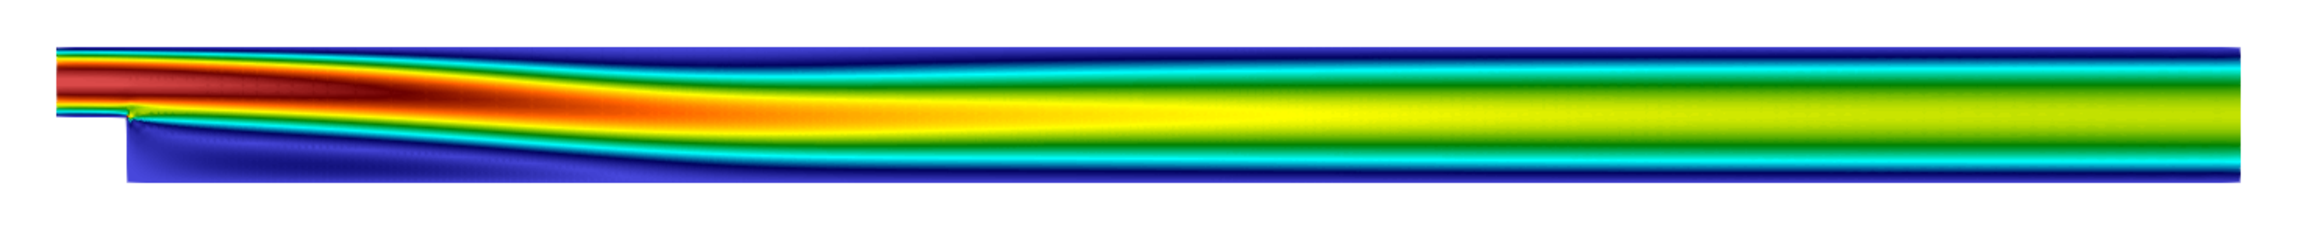
\includegraphics[scale=0.36,trim=0cm 0cm 0cm 0cm, clip=true]{Imagens/Cap3/degrau400.pdf}}\\ 
	\subfloat[\label{fig:vortice_re800}$\Reynolds= 800$]{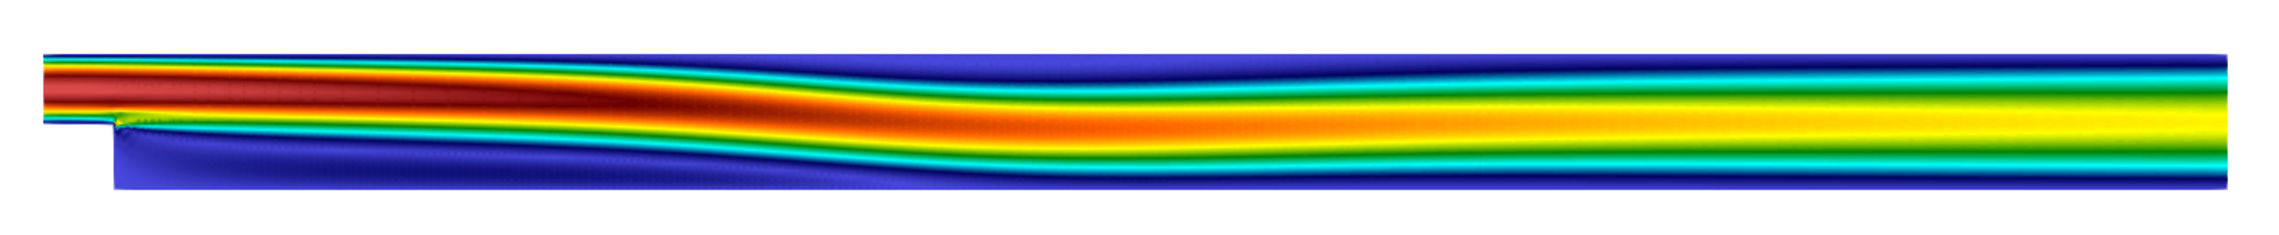
\includegraphics[scale=0.36,trim=0cm 0cm 0cm 0cm, clip=true]{Imagens/Cap3/degrau800.pdf}}\\
	{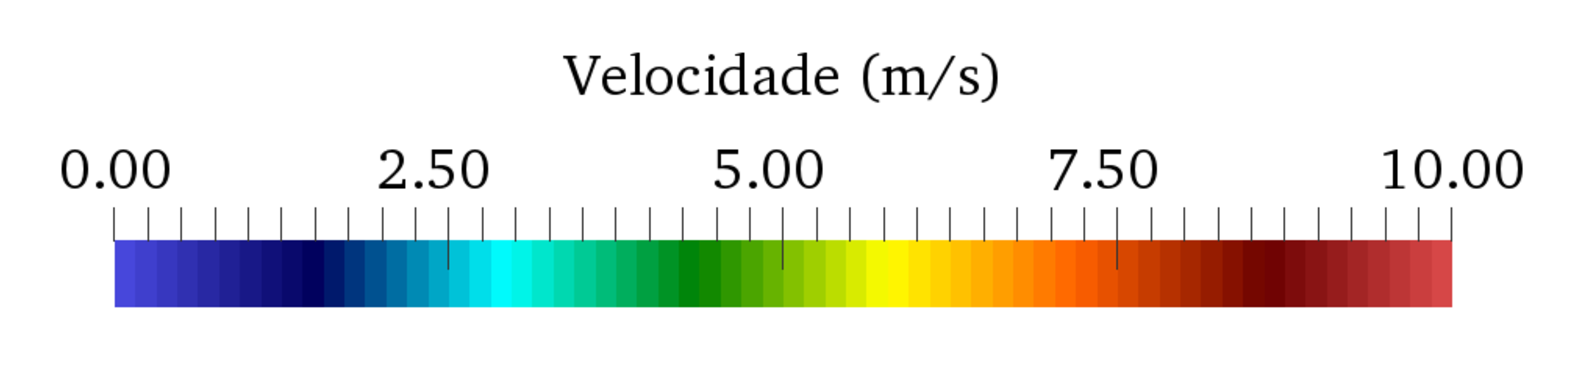
\includegraphics[scale=0.3,trim=0cm 0cm 0cm 0cm, clip=true]{Imagens/Cap3/legendadegrau.pdf}}
	\caption{Degrau 3D: Campo de velocidade. }
	\label{fig:degrau_vortices}
\end{figure}

\end{document}
